\documentclass[12pt, reqno]{amsart}

\usepackage{graphicx}
\usepackage{amssymb}
\usepackage{amsthm}
\usepackage{listings}
\usepackage{lineno}
\usepackage[margin=3cm]{geometry}
\usepackage[all,cmtip, color,matrix,arrow]{xy}
\usepackage{subfig}

%\usepackage{natbib}
%\usepackage{graphicx}
\usepackage{amsmath}%To use \text 
%\usepackage{amssymb}
%\usepackage{amsthm}
\usepackage[utf8]{inputenc}
%\usepackage[english]{babel}
%\usepackage{biblatex}
\usepackage{hyperref}
\usepackage[capitalize]{cleveref}  
\crefname{thm}{Theorem}{Theorems}
\usepackage{bbold}
\usepackage[export]{adjustbox}
%\usepackage{tikz-cd}
%\usepackage{xr}
%\usetikzlibrary{babel}
\usepackage{todonotes}
\usepackage{bm}
\usepackage{wrapfig}
\usepackage{bbold}
\usepackage{float}
\usepackage{mathtools}
\usepackage{aliascnt}
\newaliascnt{eqfloat}{equation}
\newfloat{eqfloat}{h}{eqflts}
\floatname{eqfloat}{Equation}
\usepackage{dirtytalk}

\newcommand*{\ORGeqfloat}{}
\let\ORGeqfloat\eqfloat
\def\eqfloat{%
  \let\ORIGINALcaption\caption
  \def\caption{%
    \addtocounter{equation}{-1}%
    \ORIGINALcaption
  }%
  \ORGeqfloat
}
\newcommand{\raul}[1]{\todo[color=green!30,inline]{CH, #1}}

\newcommand{\yannic}[1]{\todo[color=violet!30,inline]{YV, #1}}

\theoremstyle{definition}
\newtheorem{thm}{Theorem}[section]
\newtheorem{prop}[thm]{Proposition}
\newtheorem{lm}[thm]{Lemma}
\newtheorem{cor}[thm]{Corollary}
\newtheorem{obs}[thm]{Observation}
\newtheorem{defin}[thm]{Definition}
\newtheorem{smpl}[thm]{Example}
\newtheorem{quest}[thm]{Question}
\newtheorem{prob}[thm]{Problem}
\newtheorem{conj}[thm]{Conjecture}
\newtheorem{rem}[thm]{Remark}
\crefname{lm}{Lemma}{Lemmas}
\crefname{thm}{Theorem}{Theorems}
\crefname{prop}{Proposition}{Propositions}
\crefname{defin}{Definition}{Definitions}
\crefname{rem}{Remark}{Remarks}

\newcommand{\oPi}{\mathbf{C}}
\newcommand{\opi}{\vec{\boldsymbol{\pi}}}
\newcommand{\otau}{\vec{\boldsymbol{\tau}}}
\newcommand{\olambda}{\vec{\boldsymbol{\gamma}}}
\newcommand{\msum}{\sideset{^M}{}\sum}
\newcommand{\nestohedra}{nestohThisedra}
\newcommand{\gpHa}{\mathbf{GP}}
\newcommand{\gHa}{\mathbf{G}}
\newcommand{\citestan}{\cite[Proposition 3.2]{gebhard99}}
\newcommand{\parpi}{\boldsymbol{\pi}}
\newcommand{\partau}{\boldsymbol{\tau}}
\newcommand{\makepar}{\boldsymbol{\lambda}}
\newcommand{\uhsm}{\boldsymbol{\Psi}}
\newcommand{\uHsm}{\boldsymbol{\Psi}}
\newcommand{\sqbinom}{\genfrac{[}{]}{0pt}{}}


\newcommand{\bfpsigrf}{$\mathbf{\Psi}_{\mathbf{Q}}$}

\newcommand{\pper}{marked permutation }
\newcommand{\ppers}{marked permutations }
\newcommand{\pperp}{marked permutation.}
\newcommand{\ppersp}{marked permutations.}

\newcommand{\stirling}[2]{\genfrac{[}{]}{0pt}{}{#1}{#2}}%binomial coefficients
\newcommand{\III}{\vec{\mathbf{I}}}
\newcommand{\JJJ}{\vec{\mathbf{J}}}


\DeclareMathOperator{\w}{\mathcal{W}}
\DeclareMathOperator{\pos}{\mathrm{pos}}
\DeclareMathOperator{\s}{\mathrm{mset}}
\DeclareMathOperator{\ms}{\mathrm{mset}}
\DeclareMathOperator{\Alg}{\mathrm{Alg}}
\DeclareMathOperator{\im}{im}
\DeclareMathOperator{\id}{id}
\DeclareMathOperator{\comu}{comu}
\DeclareMathOperator{\rest}{\mathbf{res}}
\DeclareMathOperator{\Orth}{Orth}
\DeclareMathOperator{\cano}{cano}
\DeclareMathOperator{\Ppatp}{\mathbf{Ppat}^*}
\DeclareMathOperator{\dpt}{\mathbf{depth}}
\DeclareMathOperator{\pat}{\mathbf{pat}}
\DeclareMathOperator{\Pat}{\mathrm{Pat}}
\DeclareMathOperator{\Func}{\mathrm{Func}}
\DeclareMathOperator{\spn}{\mathrm{span}}
\DeclareMathOperator{\inc}{\mathrm{inc}}
\DeclareMathOperator{\Ch}{\mathrm{Ch}}
\DeclareMathOperator{\tvs}{\textvisiblespace}
\DeclareMathOperator{\sFunc}{\mathrm{SurFunc}}
\DeclareMathOperator{\End}{\mathrm{End}}
%\usepackage{lipsum}

\newcommand{\bfa}{\mathbf{a}}

%combinatorial concepts
\newcommand{\Sr}{\mathrm{S}} %symmetric group
\newcommand{\opp}[1]{\overline{#1}} %for opposite
\newcommand{\len}{l} % for length (degree) of a composition or partition
%\newcommand{\maxflat}{\hat{1}}
\newcommand{\maxflat}{\widehat{I}}
\newcommand{\minflat}{\{I\}}
\newcommand{\ifac}{
\begin{picture}(3,5)(0,0)
\put(0,0){\textup{!}}\put(1.5,4.8){\circle{3}}
\end{picture}
} %cyclic factorial
\newcommand{\acyc}[1]{#1 !} %acyclic orientations

%linear operators


%categories
\newcommand{\Fset}{\mathsf{Set^{\times}}}
\newcommand{\Veck}{\mathsf{Vec}_\Kb} 
\newcommand{\Vect}{\mathsf{Vect}} 
\newcommand{\Set}{\mathsf{Set}}
\newcommand{\Ss}{\mathsf{Sp}} % set species
\newcommand{\Ssk}{\mathsf{Sp}_\Kb} %vector species
\newcommand{\Spr}{\mathsf{Spr}} % set species with restrictions

\newcommand{\Mo}[1]{\mathsf{Mon}(#1)} %monoids
\newcommand{\Co}[1]{\mathsf{Comon}(#1)} %comonoids
\newcommand{\Bo}[1]{\mathsf{Bimon}(#1)} %bimonoids
\newcommand{\Kb}{\mathbb{K}} 



%generic set species
\newcommand{\rP}{\mathrm{P}}
\newcommand{\rQ}{\mathrm{Q}}
\newcommand{\rH}{\mathrm{H}}
\newcommand{\rR}{\mathrm{R}}


%generic species with restrictions
\newcommand{\prP}{\mathtt{P}}
\newcommand{\prQ}{\mathtt{Q}}
\newcommand{\prH}{\mathtt{H}}
\newcommand{\prR}{\mathtt{R}}


%set species
\newcommand{\rE}{\mathrm{E}}
\newcommand{\rL}{\mathrm{L}}
%\newcommand{\rX}{\mathrm{X}}
\let\rPi=\Pi %flats
\let\rSig=\Sigma
\newcommand{\rSigh}{\widehat{\rSig}} %decompositions = weak compositions
\newcommand{\rG}{\mathrm{G}} %graphs
\newcommand{\rGP}{\mathrm{GP}} %generalized permutahedra
\newcommand{\SP}{\mathfrak{p}} %standard permutahedron

%generic species
\newcommand{\thh}{\mathbf{h}} 
\newcommand{\tg}{\mathbf{g}}
\newcommand{\tk}{\mathbf{k}}
\newcommand{\tp}{\mathbf{p}} 
\newcommand{\tq}{\mathbf{q}}
\newcommand{\tr}{\mathbf{r}}
\newcommand{\ta}{\mathbf{a}}
\newcommand{\tb}{\mathbf{b}} 
\newcommand{\tc}{\mathbf{c}}
\newcommand{\td}{\mathbf{d}}
\newcommand{\trr}{\mathbf{r}} 
\newcommand{\tm}{\mathbf{m}} %module
\newcommand{\brac}{\nu} %Lie bracket

%examples of species
\newcommand{\tone}{\mathbf{1}}
\newcommand{\wU}{\mathbf{U}}
\newcommand{\wX}{\mathbf{X}}
\newcommand{\wE}{\mathbf{E}} %exponential species
\newcommand{\wL}{\mathbf{L}} %linear orders
\newcommand{\wI}{\mathbf{I}}%used in macro \tLL
\newcommand{\tLL}{\wI\hspace*{-2pt}\wL} %pairs of chambers
\newcommand{\tLie}{\mathbf{Lie}} %Lie species
\newcommand{\tPi}{\mathbf{\Pi}} %flats
\newcommand{\tSig}{\mathbf{\Sigma}} %faces
\newcommand{\tSigh}{\mathbf{\widehat{\Sigma}}} % decompositions
\newcommand{\te}{\mathbf{e}} %elements
\newcommand{\tG}{\mathbf{G}} %graphs
\newcommand{\tcG}{\mathbf{cG}} %connected graphs
\newcommand{\tGP}{\mathbf{GP}} 

%some isomorphisms
\let\isoflat=\psi
\let\isolinear=\psi
\let\isograph=\varphi


%Fock functors
\newcommand{\contra}[1]{#1^{\vee}} 
\newcommand{\Kc}{\mathcal{K}}
\newcommand{\Kcb}{\overline{\Kc}}
\newcommand{\cKc}{\contra{\Kc}}
\newcommand{\cKcb}{\contra{\Kcb}}

%functors
\newcommand{\Tc}{\mathcal{T}}
\newcommand{\Tcq}{\Tc_q}
\newcommand{\Sc}{\mathcal{S}}
\newcommand{\Pc}{\mathcal{P}} %primitive element functor
\newcommand{\Qc}{\mathcal{Q}} %indecomposables
\newcommand{\Uc}{\mathcal{U}} %universal enveloping algebra



%% natbib.sty is loaded by default. However, natbib options can be
%% provided with \biboptions{...} command. Following options are
%% valid:

%%   round  -  round parentheses are used (default)
%%   square -  square brackets are used   [option]
%%   curly  -  curly braces are used      {option}
%%   angle  -  angle brackets are used    <option>
%%   semicolon  -  multiple citations separated by semi-colon
%%   colon  - same as semicolon, an earlier confusion
%%   comma  -  separated by comma
%%   numbers-  selects numerical citations
%%   super  -  numerical citations as superscripts
%%   sort   -  sorts multiple citations according to order in ref. list
%%   sort&compress   -  like sort, but also compresses numerical citations
%%   compress - compresses without sorting
%%
%% \biboptions{comma,round}

% \biboptions{}


%\usepackage[backend=bibtex]{biblatex}
%\addbibresource{biblio.bib}

\usepackage{amsaddr}

\begin{document}

%% Title, authors and addresses
\title{Antipode formulas for pattern Hopf algebras} % Subtitle


%\author{Raul Penaguiao\footnote{\href{mailto:raulpenaguiao@sfsu.edu}{raulpenaguiao@sfsu.edu}}\footnote{Institute of Mathematics, University of Zurich, Winterthurerstrasse 190, Zurich, CH - 8057.}\footnote{{\bf Keywords:} marked permutations, presheaves, species, Hopf algebras, free algebras}\footnote{2010 AMS Mathematics Subject Classification 2010: 05E05, 16T05, 18D10}}

\author{Raul Penaguiao, Yannic Vargas}
\email{raulpenaguiao@sfsu.edu}
\email{yvargaslozada@tugraz.at}
\address{San Francisco State University}
\address{Technische Universit\"at Graz}
\keywords{permutations, presheaves, species with restrictions, species, Hopf algebras, free algebras, antipode, cancellation-free, chromatic, reciprocity}
\subjclass[2010]{05E05, 16T05, 18D10}
\date{\today} % Date

\begin{abstract}
The permutation pattern Hopf algebra is a commutative filtered and connected Hopf algebra.
Its product structure stems from counting patterns of a permutation, interpreting the coefficients as permutation quasi-shuffles.
The Hopf algebra was shown to be a free commutative algebra and to fit into a general framework of pattern Hopf algebras, via species with restrictions.

In this paper we introduce the cancellation-free and grouping-free formula for the antipode of the permutation pattern Hopf algebra.
To obtain this formula, we use the popular sign-reversing involution method, by Benedetti and Sagan.
This formula has applications on polynomial invariants on permutations, in particular for obtaining reciprocity theorems.
On our way, we also introduce the packed words patterns Hopf algebra, and present a formula for its antipode.

Other pattern algebras are discussed here, notably on parking functions, which recovers notions recently studied by Adeniran and Pudwell, and by Qiu and Remmel.
\end{abstract}


\maketitle

\tableofcontents

\section{Introduction}

In his now celebrated  ``Lemma 14'', Takeuchi (see \cite{Takeuchi1971}, Lemma 14) obtained a quite general formula for the antipode of a Hopf algebra. 
This is an antipode formula for any filtered Hopf algebra, which can be applied in much more generality and fits the framework of \textbf{pattern Hopf algebras}, which we introduce below.
However, it has been observed that it is not the most economical formula, as it leaves some cancellations to be made.

\

Economical formulas for Hopf algebras in combinatorics have played an important role in extracting old and new formulas for the objects at study, see \cite{Schmitt1993, humpert2012incidence, BS2017, aguiar2017hopf, xu2022cancellation}.
In particular, Humpert and Martin were able to explain, in \cite{humpert2012incidence}, an elusive \textit{reciprocity relation} on graphs first presented by Stanley in \cite{stanley1975combinatorial}.

\

We will introduce the reciprocity relation now.
On a graph $G$, we can define the chromatic function by counting, for each $n\geq 0$, the number of \textit{stable colourings} of its vertices, that is, colourings such that each edge is monochromatic.
This function, $\chi_G$, turns out to be a polynomial, and its degree is the number of vertices of $G$.
It makes sense to explore the evaluation $\chi_G(-1)$, and Stanley proved that this counts the \textit{acyclic orientations} of $G$.
The observation of Humpert and Martin is that $\chi$ is in fact a Hopf algebra morphism from the \textbf{incidence Hopf algebra on graphs} to the polynomial Hopf algebra, so it commutes with the antipodes of each Hopf algebra.
The antipode of the polynomial Hopf algebra is $S(x) = -x$, so the chromatic polynomial of negative numbers becomes easier to compute, via
$$\chi_G(-x) = \chi_{S(G)}(x)\, .$$

A simple formula for the antipode $S(G)$ on the incidence Hopf algebra on graphs was also presented by Humpert and Martin, where the number of acyclic orientations plays a role and explains the previous result from Stanley.
It was also used to obtain new formulas involving the Tutte polynomial.

\

A method for obtaining a cancellation-free formula that seem to work with a large family of Hopf algebras was brought forth by Sagan and Benedetti in \cite{BS2017}, called \textit{sign-reversing involution method}.
This is a classical method in enumerative combinatorics, that has found applications in fields as far as number theory. 
E.g. in \cite{zagier2009one} a new proof of the well known fact that $x^2+y^2 = p$ has integer solutions for $p$ prime whenever $p\equiv_4 1$ was presented.

\

In Hopf algebras, this method requires careful treatment of the antipode formula of Takeuchi.
However, it varies widely depending on the combinatorial Hopf algebra at hand.
Therefore, for each Hopf algebra, a new and original application of the method is needed.
Notwithstanding, this has been shown to work in the shuffle Hopf algebra, the incidence Hopf algebra on graphs and the Hopf algebras of quasisymmetric functions and multi-quasisymmetricfunctions (see \cite{BS2017}). It is still a challenging problem to find sign-reversing involutions to find cancellative-free formulas for the antipode of others classical Hopf algebras.  \footnote{In \cite{MalvenutoReutenauer}, the antipode of the Malvenuto–Reutenauer Hopf algebra was partially computed}


\

In \cite{aguiar2017hopf}, a cancellation-free antipode formula for a Hopf structure on generalized permutahedra was found. 
This has striking consequences, because several interesting combinatorial structures can be embedded in the Hopf algebra of the generalized permutahedra.
Specific examples are graphs, matroids, posets and set partitions.
Thus, this allows us to readily determine a cancellation-free formula for all these Hopf algebras.

\

Parallel to this development is the study of permutation patterns.
This is a study with roots in computer science, pioneered by Knuth in \cite{Knuth}, where a description for the \textit{stack sortable} permutations was presented via permutation patterns.
In the meantime, permutation patterns has become a well established area of expertise in combinatorics, see \cite{linton2010permutation}.

\

The second author, in \cite{Vargas}, introduced yet another tool to study permutation patterns, by building the permutation pattern Hopf algebra.
Specifically, if we consider finite sums of functions of the form 
$$ \binom{\sigma}{\pi} \coloneqq \pat_{\pi}(\tau)\coloneqq  \#\{\text{ ways to fit $\pi$ in $\tau$ }\}\, ,$$
the central functions in the study of permutation patterns, we span a vector space that is closed for pointwise product, specifically see \eqref{eq:prodperm}.
The algebra corresponding to this pointwise product is the \textbf{permutation pattern Hopf algebra} $\mathcal{A}(\mathtt{Per})$, and is shown to be free in \cite{Vargas}.

\

The construction was generalized to other combinatorial objects, in \cite{Penaguiao2020}, as long as there is a notion of restrictions, for instance graphs or marked permutations.
The resulting structures are called \textbf{pattern Hopf algebras}.
It is conjectured that all pattern Hopf algebras are free.

\

In this paper we provide a cancellation-free and grouping-free antipode formula for the pattern Hopf algebras on permutations and on packed words.
This is an application of the sign-reversing involution method.

\

We also present an original species with restrictions structure on parking functions.
This is part of a project to interpret common combinatorial objects as species with restrictions.
Crucially, objects that do not have an inherent labelling are not amenable to an interpretation as species, so this codifies an important step in this project.
The extra step here is done with a help of a new bijection between labelled Dyck paths and parking functions, introduced in \cite{BGLPV2021}.

\

The notion of patterns in parking functions here presented recovers the one presented recently in \cite{adeniran2022pattern}.
There, the authors study the number of parking functions that avoid a set of five parking functions of size three, recovering sequences like the Catalan numbers.
The original introduction of patterns in parking functions hearkens back to \cite{qiu2018patterns}.
Parking functions themselves are a recent endeavour in combinatorics, being introduced by \cite{konheim1966occupancy}, where it was shown that there are $(n+1)^{n-1}$ parking functions of length $n$.

\

In \cref{sec:antipode_computing}, we present an example of an application of the sign-reversing involution formula.
We also present some examples where we compute some antipodes via \textit{ad hoc} methods.
In \cref{sec:species} we present the algebra and category theory background to pattern Hopf algebras, and clarify the reader with the relevant Fock functors involved.
In \cref{sec:pattern_algebra_contruction}, we recall the pattern Hopf algebra construction, along with its product and coproduct structure, from a species with restrictions, so that this article is self contained.
In \cref{sec:species_restrictions}, we present several examples of species with restrictions, centrally the one on permutations, but also an original one in parking functions.
%We also present here species with restrictions on Dyck paths and on parking functions, and present simple examples of patterns in parking functions.
In \cref{sec:formula_general,sec:formula_packed,sec:formula_permutation}, we present the main result, the cancellation-free and grouping-free formula for the antipode in packed words and in $\mathcal{A}(\mathtt{Per})$.
%In this section we start by describing the sign-reversing involution method to obtain a cancellation-free formula for the antipode of a Hopf algebra.
%Then we present the main result of this section in \cref{thm:antipode_perms_intro}, a cancellation-free formula for the antipode of $\mathcal{A}(\mathtt{Per})$.


\subsection{The permutation pattern Hopf algebra and the main result}

In this section we introduce the Hopf algebra structure on permutation patterns, and present the main result on this paper.

\

Let $\pat_{\pi}$ be a function on permutations, so that $\pat_{\pi}(\sigma)$ counts the number of restrictions of the permutation $\sigma$ that fit the pattern $\pi$.
In this way, the collection of permutation pattern functions $\{\pat_{\pi}\}$ is linearly independent, so it is a basis of a vector space $\mathcal A (\mathtt{Per})$.
However, in \cite{Vargas}, it was shown that the pointwise product of two such functions can be expressed as a sum of other permutation pattern functions:
\begin{equation}\label{eq:prodperm}
\pat_{\pi_1} \pat_{\pi_2} = \sum_{\sigma} \binom{\sigma}{\pi_1, \pi_2} \pat_{\sigma} \, .
\end{equation}

The coefficients $\binom{\sigma}{\pi_1, \pi_2}$ that arise in this product formula count the so called \textbf{quasi-shuffle signatures}, or \textbf{QSS}, of $\sigma$ from $\pi_1, \pi_2$.
That is, $\binom{\sigma}{\pi_1, \pi_2}$ counts the pairs $(I, J)$ of sets that cover \yannic{Definition of ``covering''?} $\sigma$ such that $\sigma|_I = \pi_1$ and $\sigma|_J = \pi_2$.
In general, $\binom{\sigma}{\pi_1, \dots, \pi_n}$, the coefficient that arises in the iterated product of $n$ elements, counts the number of ways of covering $\sigma$ with $n$ permutations, each fitting the patterns $\pi_1, \dots, \pi_n$.

\

This algebra $\mathcal A(\mathtt{Per})$ can be endowed with a Hopf algebra structure with the help of the diagonal sum of permutations, $\oplus$, also called shifted concatenation of permutations.
If one lets $\pi = \pi_1 \oplus \dots \oplus \pi_n$ be the decomposition of $\pi$ into $\oplus$-indecomposable permutations under the $\oplus$ product, we define the shifted deconcatenation coproduct
$$\Delta \pat_{\pi} = \sum_{k=0}^n \pat_{\pi_1\oplus \dots \oplus \pi_k} \otimes \pat_{\pi_{k+1}\oplus \dots \oplus \pi_n} \in \mathcal A (\mathtt{Per}) \otimes \mathcal A (\mathtt{Per})\, .$$

\begin{thm}[Antipode formula for Permutation pattern Hopf algebra]\label{thm:antipode_perms_intro}
Let $\pi = \pi_1\oplus \dots \oplus \pi_n$ be a decomposition of a permutation $\pi$ into $\oplus$-indecomposable permutations.
Then, we have the following formula for the antipode of $\pat_{\pi}$:

$$S(\pat_{\pi}) = (-1)^n \sum_{\sigma} \bigl[\!\begin{smallmatrix} \omega \\ \pi_1, \dots, \pi_n \end{smallmatrix}\!\bigr] \pat_{\sigma}\, ,$$
where the sum runs over all permutations $\sigma$, and the coefficients count the number of \textbf{interlacing QSS} of $\sigma$ from $\pi_1, \dots, \pi_n$.
\end{thm}

As in the case of graphs, this antipode formula has consequences in polynomial invariants.
These are discussed in \cite{Penaguiao2020}.

\

We present a definition of interlacing QSS below, along with some examples that help discern this notion.
We also present an antipode formula for the packed words pattern Hopf algebra, with a similar characterization. \yannic{In the following, the definition of QSS is presented, inside an example. Should it be in an independent Definition?}

\

\begin{smpl}[Interlacing QSS]
A quasi-shuffle signature, or a QSS, of $\sigma $ from $\pi_1, \dots, \pi_n$ is a sequence of sets $\III = (I_1, \dots, I_n)$ that cover $\sigma$ such that $\sigma|_{I_i} = \pi_i$.
This QSS is said to be \textbf{non-interlacing} if there is some $i=1, \dots, n-1$ such that $I_i < I_{i+1}$ and $\sigma(I_i) < \sigma(I_{i+1})$.
Otherwise, we say that the QSS is \textbf{interlacing}. 
\begin{figure}[h]
    \centering
    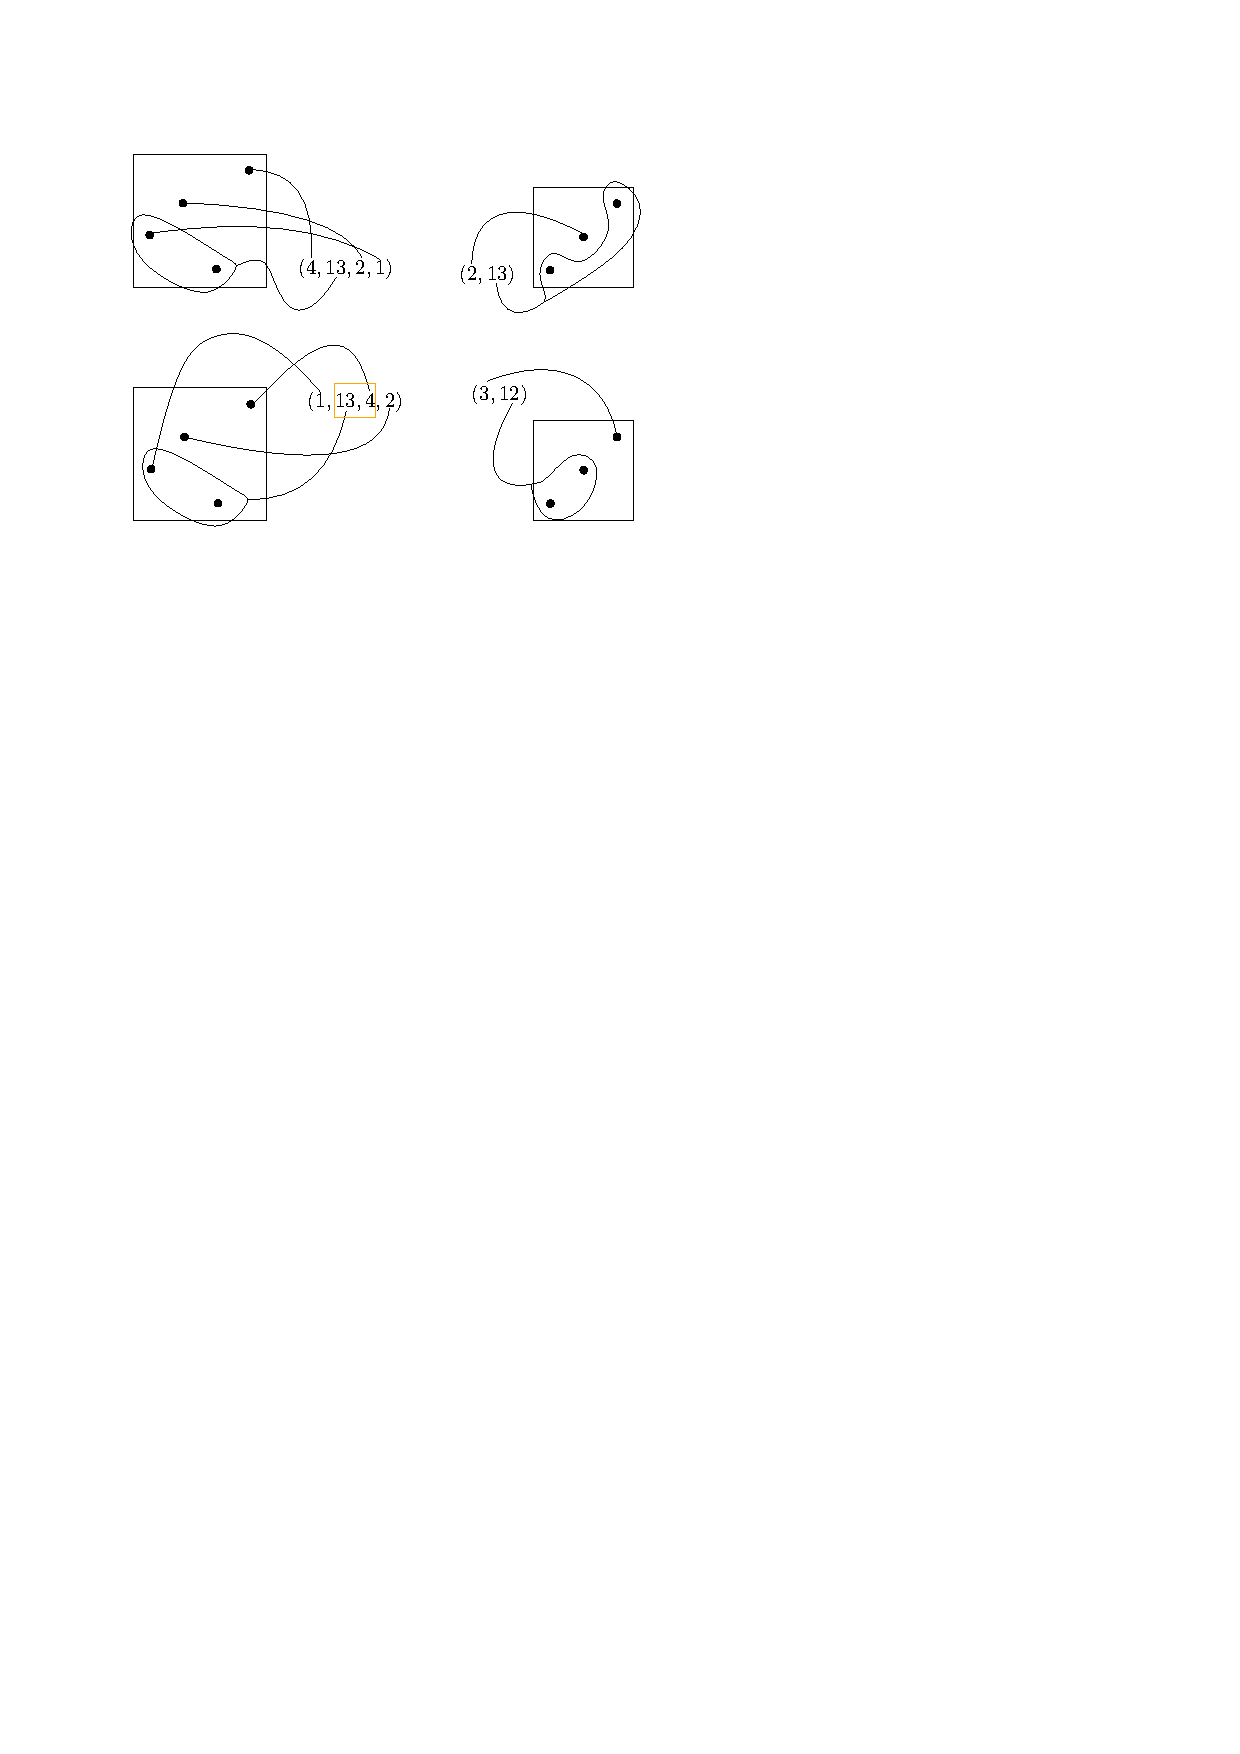
\includegraphics{images/interlacing_25314.pdf}
    \caption{\textbf{Left:} the permutation 2314, along with a labelling of two of its QSS from $21, 1, 1, 1$. In orange the two sets that do not interlace. \textbf{Right:} the permutation 123, along with its two interlacing QSS from $1, 12$.\label{fig:interlacingQSSsmpl}}
\end{figure}

\

So the permutation $2314$ has several QSS from $1, 21, 1, 1$, for instance $(4, 13, 2, 1)$ and $(1, 13, 4, 2)$, but from these two, only the first is interlacing.
In \cref{fig:interlacingQSSsmpl}, one can see these two QSS.
Further computations can show that $\binom{2314}{1, 21, 1, 1} = 36$ and $\bigl[\!\begin{smallmatrix} 2314 \\ 1, 21, 1, 1 \end{smallmatrix}\!\bigr] = 8$.

One can observe that there are three QSS of $123$ from $1$, $12$, but one of them is non-interlacing (the QSS $(1,23)$), so
$\bigl[\!\begin{smallmatrix} 123 \\ 1, 21 \end{smallmatrix}\!\bigr] = 2$.
In \cref{fig:interlacingQSSsmpl}, one can see these two interlacing QSS.
\end{smpl}


\section{Computing the antipode\label{sec:antipode_computing}}

We will now explore the classical methods to obtain the antipode, using basic axioms and the Takeuchi formula, on the polynomial algebra and on the permutation pattern Hopf algebra.
These methods fail to give a cancellation-free and grouping-free formula for the antipode.

We start by recalling Takeuchi's formula, in the form that is presented in \cite{GrinbergReiner}.
%This is the beginning of any cancellation-free formula.

Let us define the $\star$ notation on maps $a, b: C \to A$, whenever $A$ is an algebra, and $C$ is a coalgebra, we define:
$$a \star b \coloneqq \mu_A \circ (a \otimes b) \circ \Delta_C\, ,$$
which defines an associative and unitary product on linear maps from $C$ to $A$. We will be focused on the case when $C=A=H$ is a Hopf algebra, so this defines an operation on $\End(H)$.

\begin{prop}[Takeuchi's formula, Lemma 14]\label{lm:takeuchi}
If $H = (H, \mu, \iota, \Delta, \epsilon, S)$ is a Hopf algebra such that $(\epsilon\circ \iota - \id_H)$ is $\star$-nilpotent, then 
\begin{equation}\label{eq:eq1}
S = \sum_{k\geq 0 }  ( \iota  \circ\epsilon- \id_H)^{\star k} = \sum_{k\geq 0} (-1)^k \mu^{\circ (k-1)} \circ (\id_{H} - \iota \circ \epsilon)^{\otimes k} \circ \Delta^{\circ (k-1)}\, .
\end{equation}

We use the convention that $\Delta^{\circ (-1)} = \epsilon $ and $\mu^{\circ (-1)} = \iota$.
\end{prop}

Note that, for any filtered Hopf algebra, $( \iota \circ \epsilon - \id_H)$ is $\star$-nilpotent.
Therefore, for any pattern algebra, Takeuchi's formula holds.
This is summarized in \cref{thm:conHopfalgebra}.

\

In the Hopf algebra of polynomials, this gives us the following:
$$S(x^3) = \underbrace{0}_{k = 0} - \underbrace{x^3}_{k = 1} + \underbrace{3 x^2 \cdot x + 3 x \cdot x^2}_{k=2} - \underbrace{6 x \cdot x \cdot x}_{k = 3} = - x^3 \, .$$


We now present another example, this time on the permutation pattern Hopf algebra $\mathcal A(\mathtt{Per})$.
Consider $\pi = 132 = 1 \oplus 21$. Then Takeuchi's formula gives us:
\begin{align*}
S(\pat_{132}) =& \sum_{k=0}^2 (-1)^k \mu^{\circ k-1} \circ (\id_{\mathcal A(\mathtt{Per})} - \iota \circ \epsilon)^{\otimes k} \circ \Delta^{\circ k-1}(\pat_{132})\\
=& -(\id_{\mathbb{K}[x]} - \iota \circ \epsilon)(\pat_{132}) + \mu \circ (\id_{\mathbb{K}[x]} - \iota\circ\epsilon)^{\otimes 2}(\pat_1 \otimes \pat_{12}) \\
=& \underbrace{0}_{k = 0} - \underbrace{\pat_{132}}_{k=1} + \underbrace{\pat_1 \pat_{21}}_{k=2} \\
=& 3 \pat_{321} + 2 \pat_{231} + 2 \pat_{312} + \pat_{213} + 2 \pat_{21} \, .
\end{align*}

\

These coefficients can be seen as enumerating quasi-shuffle signatures of $132$ from $1$ and $12$ that are \textbf{interlacing}, according to \cref{thm:antipode_perms_intro}.



\

\subsection{The sign-reversing involution method}

The application of the sign-reversing involution method to compute antipodes of Hopf algebras was first presented in \cite{BS2017}.
This is a method to find cancellation-free formulas for the antipode of a Hopf algebra.
It starts in the formula given by Takeuchi, and keeps track of all the terms to be summed, usually by means of compositions, that arise in this formula.
Thus, the sum obtained runs over a collection of objects, say $\mathcal O$, that is partitioned into families indexed by compositions.
These compositions play an important role in the sum, as their length determines the sign of the corresponding objects.

\

Recall that an involution $\zeta $ is an endomorphism such that $\zeta \circ \zeta$ is the identity.
We describe an involution in $\mathcal O$, call it $\zeta $, in such a way that if $\zeta(x) \neq x$, then $x$ and $\zeta(x)$ contribute with opposite signs to the antipode.
As a consequence, when applying Takeuchi's formula, we can cancel terms that are not fixed points of $\zeta$.
We give an example of how this method is applied in the Hopf algebra $\mathbb{K}[x]$.

\

The following is a computation from \cite{BS2017}.
We would like to point out that there are easier ways to obtain an antipode formula for the polynomial Hopf algebra: the interested reader can find some for instance in \cite{GrinbergReiner}.
However, it shows the power of Takeuchi’s formula, as the whole process can be done with little recourse to intuition.


\begin{thm}[The antipode formula for the polynomial Hopf algebra]\label{thm:polyHA}
The antipode $S$ for $\mathbb{K}[x] $ is 
$$ S(x^n) =(-x)^n\, . $$
\end{thm}

To prove this formula, we first introduce \textit{weak compositions}.
A \textbf{weak composition} $\alpha$ of an integer $n$ is a list of non-negative integers $\alpha = (\alpha_1, \dots , \alpha_l)$ such that $\sum_i \alpha_i = n$.
We denote the length of the weak composition by $l = l(\alpha)$, and use the shorthand notation $\alpha \models^0 n$.
If $\alpha $ has no zero entries, we say that $\alpha$ is a \textbf{composition}, and write $\alpha \in \mathcal C_n$.

\

A \textbf{weak set composition} $\opi$ of a set $A$ is a list of sets $\opi = (A_1, \dots , A_l)$ such that $\biguplus_i A_i = A$.
Note that some sets may be empty.
We denote the length of the weak composition by $l= l(\opi)$, and use the shorthand notation $\opi \models^0 A$.
If the weak set composition does not contain any empty set, we say that is a \textbf{set composition}, and we denote $\opi \models A$.
There are finitely many set compositions of a given set $A$, whereas there are infinitely many weak set compositions of $A$.
Let $\mathbf{C}_A$ be the collection of set composition of $A$.
We abbreviate to $\mathbf{C}_n$ when $A = [n]$.

\begin{proof}[Proof of \cref{thm:polyHA}]
We use Takeuchi formula, given in \eqref{eq:eq1}, which holds for graded Hopf algebras,
$$S(x^n) = \sum_{k = 0} (-1)^k \mu^{\circ (k-1)} \circ (\id_{\mathbb K[x]} - \iota \circ \epsilon )^{\otimes k} \circ \Delta^{\circ (k-1)} (x^n) \, .$$

The key observation on the sign-reversing involution method is to reshuffle this sum using:
$$ \Delta^{\circ (k-1) } (x^n) = \sum_{(A_1, \dots , A_k) \models^0 [n] } x^{|A_1|} \otimes \dots \otimes x^{|A_k|} \, ,$$
where the sum runs over weak set compositions of the set $[n]$ with size $k$.
This can be shown with easy induction on $n$.
Thus, the antipode formula can be rewritten as

\begin{align*}
S(x^n)&= \sum_{k=0}^n(-1)^k \sum_{(A_1, \dots , A_k) \models^0 [n]} \mu^{\circ (k-1)} \circ (\id_{\mathbb K[x]} - \iota \circ \epsilon )^{\otimes k} (x^{|A_1|} \otimes \dots \otimes x^{|A_k|})   \\
	  &= \sum_{k=0}^n(-1)^k \sum_{(A_1, \dots , A_k) \models [n]} \mu^{\circ (k-1)} (x^{|A_1|} \otimes \dots \otimes x^{|A_k|})   \\
	  &= \sum_{k=0}^n(-1)^k \sum_{(A_1, \dots , A_k) \models [n]} x^n   \\
	  &= x^n \sum_{\opi \models [n]} (-1)^{l(\opi)}\, .
\end{align*}

Consider the following involution $\zeta: \oPi_{n} \to \oPi_{n} $.
For $\opi = (A_1, \dots , A_k) $, let $j_{\opi}$ be the smallest index such that $|A_{j_{\opi}}| \neq 1$ or $\max A_{j_{\opi}} > \max A_{j_{\opi}+1} $.
Then, there are three cases:

\begin{enumerate}

\item The set $A_{j_{\opi}} $ is a singleton with $j\leq k-1$, then let $\zeta(\opi ) $ be the set composition resulting from merging $A_{j_{\opi}} $ and $A_{j_{\opi}+1}$.
Note how, in this case, $\max A_{j_{\opi}} \cup A_{j_{\opi} + 1} $ is the only element in $A_{j_{\opi}}$.

\item The set $A_{j_{\opi}} $ is not a singleton, then we define $\zeta(\opi ) $ to be the set composition resulting from splitting $A_{j_{\opi}} $ into $\{ \max A_{j_{\opi}} \} $ and $A_{j_{\opi}} \setminus \{\max A_{j_{\opi}} \}$, in this order.

\item There is no such $j_{\opi}$. Then $\opi = (\{1\}, \dots , \{n\})$ and we define $\zeta(\opi )= \opi $.

\end{enumerate}

It is a direct observation that $\zeta $ is an involution.
In fact, the only fixed point is $\opi = (\{1\}, \dots , \{n\})$, and for any other set composition $\opi$, whenever the index $j_{\opi}$ in $\opi $ behaves as described in case 1, then the index $j_{\zeta(\opi)}$ in $\zeta ( \opi ) $ behaves as described in case 2, in which case we have $l(\opi) = 1+l(\zeta (\opi))$ and we can easily see that $\zeta(\zeta(\opi )) = \opi$.
We also have the converse statement. Thus, we have that 
\[x^n \sum_{\opi \in \oPi_n} (-1)^{l(\opi)} = x^n (-1)^{l(\{1\}, \dots, \{n\} )}= (-x)^n,\] 
as desired.
\end{proof}


In this way we see that a formula for the antipode depends simply on an understanding of the structure of the length of compositions of $[n]$.
This is a general feature whenever we apply Takeuchi's formula.





\

\section{Species, species with restrictions\label{sec:species}}


In this section we will give the preliminaries of monoids in species.
This will follow closely \cite{AM2010} and \cite{Schmitt1993}.
Specifically, we will introduce species with vector spaces and sets.
We will also introduce species with restrictions, and we will clarify the meaning of a monoid, comonoid, bimonoid and Hopf monoid in each of these monoidal categories.
We will finally present some examples of species with restrictions that will be important in the remaining paper. 

\subsection{Species}
In this section we recall the basic definitions of the general theory of \emph{combinatorial species}. Following \cite{AM2010}, we will focus first in \emph{vectorial species} and \emph{set species}.

\

Let $\mathbb{k}$ be a field of arbitrary characteristic. Let $\Fset$ be the category of finite sets and bijections between finite sets, and $\Vect_{\mathbb{K}}$ be the category of $\mathbb{K}$-vector spaces and linear maps between vector spaces. A {\bf vector species}, or simply a \textbf{species}, is a functor $\tp: \Fset \to \Vect_{\mathbb{K}}$. A morphism between species $\tp$ and $\tq$ is a natural transformation between the functors $\tp$ and $\tq$.
We will always denote the vector species with a bold lowercase Latin letter, with few exceptions.

\

A species $\tp$ is said {\bf positive} is $\tp[\emptyset]=0$. The {\bf positive part} of a species $\tq$ is the positive species $\tq_+$ given by
\[\tq_+[I]=\begin{cases}
\tq[I],& \text{ if } I\neq \emptyset\\
\emptyset, & \text{ otherwise}
\end{cases}.\]

Given a vector space $V$, let ${\bf 1}_V$ be the vector species defined by
\[{\bf 1}_V[I]=\begin{cases}
V,& \text{ if } I= \emptyset\\
\emptyset, & \text{ otherwise}
\end{cases}.\]

\

We write $\Ss_{\mathbb{K}}$ for the category of vector species over the field $\mathbb{K}$. There are several possible monoidal structures on this category. 
We will consider two of them: the {\bf Cauchy} and {\bf substitution} products $\cdot$ and $\circ$, respectively: for any finite set $I$,
\[(\tp \cdot \tq)[I]:=\bigoplus_{I = S \sqcup T}\tp[S]\otimes \tq[T];\]
\[(\tp \circ \tq)[I]:=\bigoplus_{X \vdash I}\tp[X]\otimes \left(\bigotimes_{B \in X} \tq[S] \right).\]

We denote by $(\Ssk, \cdot)$ and $(\Ssk, \circ)$ the resulting monoidal categories obtained from the Cauchy and substitution operations, respectively.

\

We can also consider {\bf set species}, whose are simply functors $\rP: \Fset \to \Set$, where $\Set$ is the category of arbitrary sets and arbitrary maps between sets. Given a set species $\rP$, the notions of {\bf positive part} $\rP_+$ of $\rP$, {\bf positive set species} are defined analogously as for vector species. If $C$ is a set, let ${\bf 1}_C$ be the set species defined by
\[{\bf 1}_C[I]=\begin{cases}
C,& \text{ if } I= \emptyset\\
\emptyset, & \text{ otherwise}
\end{cases},\]
for any finite set $I$.
We will always denote a set species with a capital Latin letter, with few exceptions.

\

The Cauchy and substitution products of vector species have their analogues in this context. For instance, if $\rP$ and $\rQ$ are two set species, let
\[(\rP \cdot \rQ)[I]:=\bigsqcup_{I = S \sqcup T}\rP[S]\times \rQ[T];\]
\[(\rP \circ \rQ)[I]:=\bigsqcup_{X \vdash I}\rP[X]\times \left(\prod_{B \in X} \rQ[S] \right),\]
on any finite set $I$, where the $\times$ symbol in the right-hand sides refers to the Cartesian product.
We write $(\Ss, \cdot)$ for the monoidal category of set species.

\

It is possible to relate set species to vector species via the \emph{linearization functor} $\mathbb{K}(-): \Set \to \Vect_{\mathbb{K}}$, which sends a set to the vector space generated by the given set. Composing a set species $\rP$ with the linearization functor gives a vector species, denoted by $\mathbb{k}\rP$. A {\bf linearized species} is a vector species $\tp$ of the form $\tp=\mathbb{k}\rP$, for some set species $\rP$. We have natural isomorphisms
 \[\mathbb{K}(\rP \cdot \rQ)\simeq \mathbb{K}\rP \cdot \mathbb{K}\rQ \qquad , \qquad \mathbb{K}(\rP \circ \rQ)\simeq \mathbb{K}\rP \circ \mathbb{K}\rQ.\]

\

\subsection{Algebraic structures on vector species}


\subsubsection{Monoids}
A {\bf monoid} in $(\Ssk, \cdot)$  consist of a species $\tp$ equipped with morphisms of species
\begin{equation*}
    \mu: \tp \cdot \tp \to \tp \qquad \text{ and } \qquad \iota: \mathrm{1}_{\mathbb{K}} \to \tp.
\end{equation*}

That is, for each finite set $I$ and for each decomposition $I=S \sqcup T$, we have a linear map 
\begin{equation*}
    \mu_{S,T}: \tp[S] \otimes \tp[T]\to \tp[I] \text{ and } \iota_\emptyset: \mathbb{K} \to \tp[\emptyset].
\end{equation*}

If $x \in \tp[S]$, $y \in \tp[T]$,  let 
\[x \cdot y \in \tp[I]\]
denote the image of $x\otimes y$ under $\mu_{S,T}$. 

\

The collection of linear maps $\mu=(\mu_{S,T})$, called the {\bf product} of the monoid, must satisfy the following axioms.

\

\begin{itemize}
    \item[(i)] Naturality axiom: for finite sets $I,J$, a bijection $\sigma: I \to J$, a decomposition $I=S \sqcup T$ and elements $x \in \tp[S]$ and $y \in \tp[T]$, we have
\begin{equation*}
\tp[\sigma](x \cdot y)=\tp[\sigma(S)](x) \cdot \tp[\sigma(T)](y) \, .
\end{equation*}

\item[(ii)] Associativity axiom: for finite set $I$, a decomposition $I=R \sqcup S \sqcup T$ and for elements $x \in \tp[R]$, $y \in \tp[S]$ and $z \in \tp[T]$, we have
\begin{equation}\label{eq:axiomii}
    (x \cdot y)\cdot z=x \cdot (y \cdot z).
\end{equation}

\item[(iii)] Unit axiom: for each finite set $I$ and $x \in \tp[I]$, we have
\begin{equation*}
 x \cdot \iota_\emptyset(1) = x =  \iota_\emptyset(1) \cdot x,
\end{equation*}
where $1\in \mathbb{K}$ is the unit of the filed $\mathbb{K}$.

\end{itemize}


\

A monoid $(\tp, \mu, \iota)$ in $(\Ssk, \cdot)$ is {\bf commutative} if
\begin{equation*}
    x\cdot y=y\cdot x,
\end{equation*}
for all $I=S \sqcup T$, $x \in \tp[S]$ and $y \in \tp[T]$.

\

Let $(\tp, \mu, \iota)$ be a monoid. From the associativity axiom, for any decomposition $I=S_1 \sqcup \cdots \sqcup S_k$ with $k \geq 2$ there is a unique map
\begin{equation}
    \mu_{S_1, \hdots, S_k}: \tp[S_1]\otimes \cdots \otimes \tp[S_k] \to \tp[I],
\end{equation}
called the {\bf higher product map} of $\tp$, obtained by iterating the product maps in any meaningful way. 
This is well defined from \eqref{eq:axiomii}.
We can extend the definition of higher product map for all $k\geq 0$: for $k=1$, $\mu_I$ is defined as the identity map of $\tp[I]$ ($I$ is the only decomposition of itself in one block); if $k=0$, then $\mu_{\empty}:=\iota_{\empty}$.
Note how in this case $I = \emptyset $.
\

Monoids are closed under the Cauchy product. Also, if $(\tp, \mu, \iota)$ is a monoid, then $\tp[\emptyset]$ is an algebra with product $\mu_{\emptyset, \emptyset}$ and unit $\iota_\emptyset(1)$ (see \cite{AM2013}, section 2.3).


\

\subsubsection{Comonoids}
A {\bf comonoid} in $(\Ssk, \cdot)$ corresponds to the dual notion of monoids in $(\Ssk, \cdot)$. Formally, a comonoid consists of a species $\tp$ equipped with morphisms of species
\begin{equation*}
    \Delta: \tp \to \tp \cdot \tp \qquad \text{ and } \qquad \varepsilon: \tp \to 1_{\mathbb{K}}.
\end{equation*}

That is, for each finite set $I$ and for each decomposition $I=S \sqcup T$, we have a linear map 
\begin{equation*}
    \Delta_{S,T}: \tp[I] \to \tp[S] \otimes \tp[T] \text{ and } \varepsilon_\emptyset: \tp[\emptyset] \to \mathbb{K}.
\end{equation*}

\

The collection of linear maps $\Delta=(\Delta_{S,T})$, called the {\bf coproduct} of the monoid, must satisfies the following axioms.

\

\begin{itemize}
    \item[(i)] Naturality axiom: for finite sets $I, J$, bijection $\sigma: I \to J$, a decomposition $I = S \sqcup T$ and an element $x\in \tp [I]$.
\begin{equation*}
(\tp[\sigma|_S] \otimes \tp[\sigma|_T])\circ\Delta_{S,T}(x)=\Delta_{\sigma(S), \sigma(T)} \circ\tp[\sigma](x).
\end{equation*}

\item[(ii)] Coassociativity axiom: for a finite set $I$, a decomposition $I=R \sqcup S \sqcup T$ and for each $x \in \tp[I]$, we have
\begin{equation}\label{eq:coaxiomii}
    (\Delta_{R,S}\otimes \text{id}_{\tp[T]})\circ \Delta_{R \sqcup S, T}(x)=(\text{id}_{\tp[R]} \otimes \Delta_{S,T})\circ \Delta_{R, S \sqcup T}(x).
\end{equation}
\vspace{.1in}
\item[(iii)] Counit axiom: for each finite set $I$ and $x \in \tp[I]$, we have
\begin{equation*}
(\varepsilon_\emptyset \otimes \text{id}_{\tp[I]})\circ\Delta_{\emptyset, I}(x)= x = (\text{id}_{\tp[I]} \otimes \varepsilon_\emptyset)\circ\Delta_{I,\emptyset}(x).
\end{equation*}

\end{itemize}


\

A comonoid $(\tp, \mu, \iota)$ in $(\Ssk, \cdot)$ is {\bf cocommutative} if for any finite disjoint sets $S, T$, and element $x\in \tp[S\sqcup T]$, we have
\begin{equation*}
    \Delta_{S,T}(x)=\Delta_{T,S}(x).
\end{equation*}

\

Let $(\tp, \mu, \iota)$ be a comonoid. Dually to the case of monoids, every decomposition $I=S_1 \sqcup \cdots \sqcup S_k$ with $k \geq 0$ gives rises to a unique linear map
\begin{equation}
    \Delta_{S_1, \hdots, S_k}: \tp[I] \to \tp[S_1]\otimes \cdots \otimes \tp[S_k],
\end{equation}
called the {\bf higher coproduct map} of $\tp$, obtained by iterating the coproducts map $\Delta_{S,T}$. 
This is well defined because of \cref{eq:coaxiomii}.
çwe extend this definition to $k=1$ as the identity of $\tp[I]$ and for $k=0$, this map is the counit map $\varepsilon_\emptyset$.

\

Comonoids are closed under the Cauchy product. 
If $(\tp, \Delta, \varepsilon)$ is a comonoid, then $\tp[\emptyset]$ is a coalgebra with coproduct $\Delta_{\emptyset, \emptyset}$ and counit $\varepsilon_\emptyset$ (see \cite{AM2013}, section 2.4).

\

\subsubsection{Bimonoids  and Hopf monoids}
A {\bf bimonoid} $(\thh, \mu, \Delta, \iota, \varepsilon)$ in $(\Ssk, \cdot)$ is a monoid and comonoid such that the diagram
\[\xymatrix{
\thh[A] \otimes \thh[B] \otimes \thh[C] \otimes \thh[D] \ar[rr]^-{\cong} && \thh[A] \otimes \thh[C] \otimes \thh[B] \otimes \thh[D] \ar[dd]^-{\mu_{A,C}\otimes\mu_{B,D}}\\
&&\\
\thh[S_1]\otimes \thh[S_2]\ar[uu]^-{\Delta_{A,B}\otimes \Delta_{C,D}} \ar[r]_-{\mu_{S_1, S_2}} & \thh[I] \ar[r]_-{\Delta_{T_1, T_2}} & \thh[T_1]\otimes \thh[T_2]
}\]

commutes, where $I=S_1\sqcup S_2=T_1 \sqcup T_2$ are two decompositions of a finite set $I$ with the following resulting pairwise intersections:
\[A:=S_1\cap T_1 \quad , \quad B:=S_1 \cap T_2 \quad , \quad C:=S_2 \cap T_1 \quad , \quad D:=S_2 \cap T_2.\]
This is also schematically presented in \cref{fig:bimonoid}.


\begin{figure}
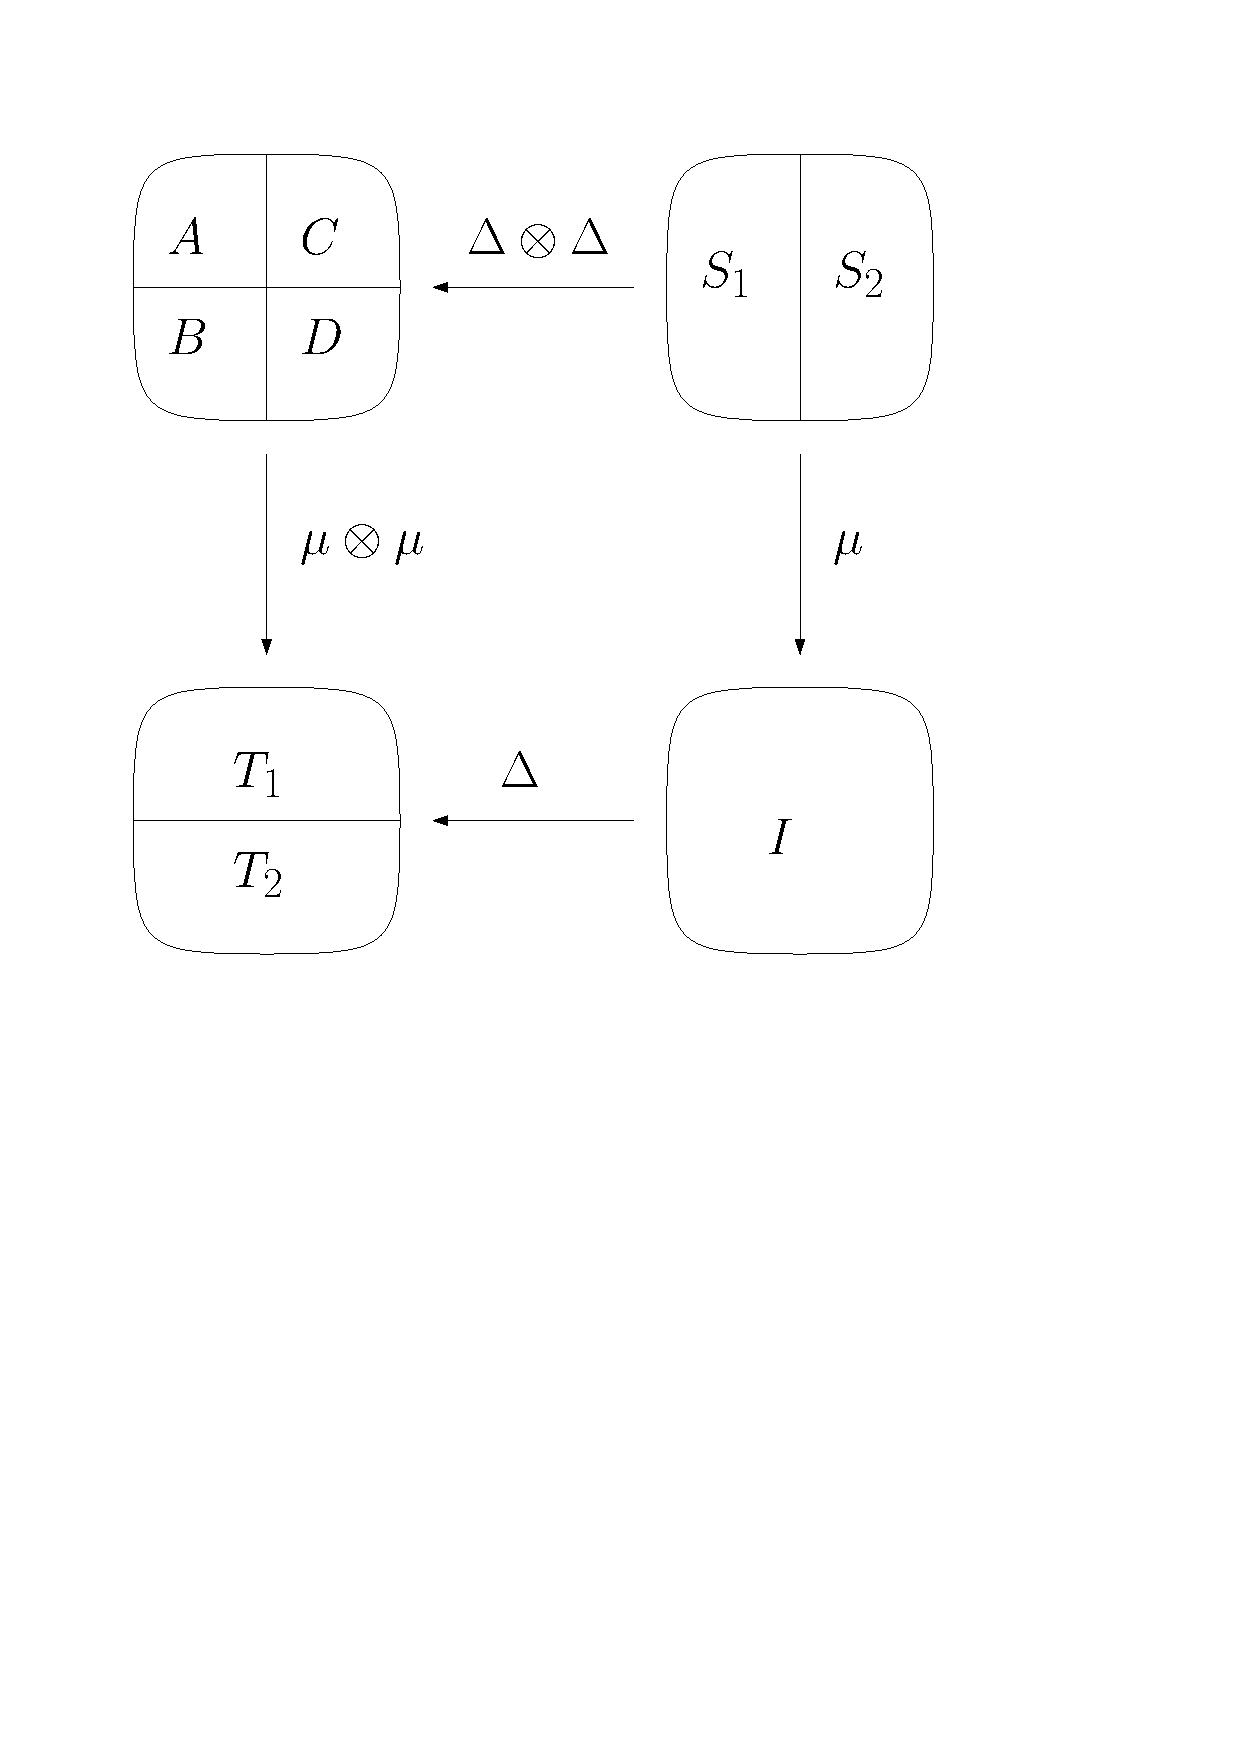
\includegraphics[scale=0.5]{images/diagram_bialgebra}
\caption{The bimonoid compatibility axiom.\label{fig:bimonoid}}
\end{figure}

\

We can define the convolution algebra $\text{End}_{\Ssk}(\thh)$ as the set of natural transformations $l: \thh \to \thh$ with the product $\star$.

A morphism of species $s: \thh \to \thh$, is callen and {\bf antipode} of $\thh$, if $\thh[\emptyset]$ is a Hopf algebra with antipode $s_\emptyset: \thh[\emptyset] \to \thh[\emptyset]$, and for each nonempty set $I$, we have
\begin{equation}
    \sum_{S \sqcup T = I} \mu_{S,T}(\text{id}_S \otimes s_T)\Delta_{S,T} = 0 = \sum_{S \sqcup T = I} \mu_{S,T}(s_S \otimes \text{id}_T)\Delta_{S,T}.
\end{equation}

A {\bf Hopf monoid} in $(\Ssk, \cdot)$ is a bimonoid along with an antipode $s:\thh \to \thh $.
Equivalently, the identity map $\text{id}_{\thh}$ is invertible in $\text{End}_{\Ssk}(\thh)$ (c.f. \cite{AM2010}, section 2.7).
Recall that this is also the case in the classical Hopf algebras.
\

\subsection{Algebraic structures on set species}

The notions of monoid, comonoid, bimonoid and Hopf monoid for set species can be described in terms similar to those in the previous section. 

\

\subsubsection{Monoids}
A {\bf monoid in set species} consist of a species $\rP$ equipped with morphisms of species
\begin{equation}
    \mu: \rP \cdot \rP \to \rP \qquad \text{ and } \qquad \iota: \mathrm{1}_{\{\emptyset \} } \to \rP.
\end{equation}

That is, for each decomposition $I=S \sqcup T$, we have maps 
\begin{equation}
    \mu_{S,T}: \rP[S] \times \rP[T]\to \rP[I] \text{ and } \iota_\emptyset: \{\emptyset\} \to \rP[\emptyset].
\end{equation}

If $x \in \rP[S]$, $y \in \rP[T]$,  let 
\[x \cdot y \in \rP[I]\]
denote the image of $(x,y)$ under $\mu_{S,T}$. Also, let $e\in \rP[\emptyset]$ denote the image of $\emptyset$ under $\iota_\emptyset$.

\

The collection of maps $\mu=(\mu_{S,T})$, called the {\bf product} of the monoid, must satisfies naturality, associativity and unit axioms analogue to the ones defined for monoids in vector species.

\

Note that, for any monoid on a set species $(\rP, \mu, \iota)$, then $(\rP[\emptyset], \mu_{\emptyset, \emptyset}, \iota_\emptyset)$ is a set theoretical monoid.

\

A monoid in set species $(\rP, \mu, \iota)$ is {\bf commutative} if
\[x\cdot y=y\cdot x,\]
for all $I=S \sqcup T$, $x \in \rP[S]$ and $y \in \rP[T]$.

\

\subsubsection{Comonoids}
A {\bf comonoid in set species} consist of a species $\rP$ equipped with morphisms of species
\[\Delta:\rP \to \rP \cdot \rP \qquad \text{ and } \qquad \varepsilon: \rP \to \mathrm{1}_{\{\emptyset \} }. \]
That is, for each decomposition $I=S \sqcup T$ we have maps $\Delta_{S,T}: \rP[I]\to \rP[S] \times \rP[T]$, and $\varepsilon_\emptyset: \rP[\emptyset] \to \{\emptyset\}$. If $x \in \rP[I]$,  let 
\[(x|_S, x /_S)\in \rP[S]\times \rP[T]\]
denote the image of $(x,y)$ under $\Delta_{S,T}$. The map $x \mapsto x|_S$ can be thought as a ``restriction'' of the structure $x$ from $I$ to $S$, while $x \mapsto x/_S$ can be associated to a ``contraction'' of $S$ from $x$, resulting in a structure on $T$.

\

The collection of maps $\Delta=(\Delta_{S,T})$, called the {\bf coproduct} of the monoid, must satisfy naturality, coassociativity and counit axioms analogues to the ones defined for monoids in vector species. In terms of the restriction/contraction notation, these axioms are described as follows:
\begin{itemize}
    \item Naturality axiom: for each bijection $\sigma: I \to J$,  we have
\[{\Big (}\rP[\sigma](x){\Big )}|_{\sigma(S)}=\rP[\sigma|_S](x|_S) \qquad , \qquad {\Big (}\rP[\sigma](x){\Big )}/_{\sigma(S)}=\rP[\sigma|_T](x/_S),\]
for all $x \in \rP[I]$.
\vspace{.1in}
\item Coassociativity axiom: for all decomposition $I=R \sqcup S \sqcup T$, \[(x|_{R\sqcup S})|_R=x|_R \qquad , \qquad (x|_{R\sqcup S})/_R=(x/_R)|_S \qquad , \qquad x/_{R \sqcup S}=(x/_R)/_S, \]
for all $x \in \rP[I]$
\vspace{.1in}
\item Counit axiom: we have
\[x|_I= x = x/_\emptyset,\]
for each finite set $I$ and for each $x \in \rP[I]$. In particular, $\Delta_{\emptyset, \emptyset}(x)=(x,x)$, for each $x \in \rP[\emptyset]$.
\end{itemize}

\


A comonoid in set species $(\rP, \Delta, \varepsilon)$ is {\bf cocommutative} if
\[x|_S=x/_T,\]

for any disjoint finite sets $S, T$ and $x \in \rP[S\sqcup T]$.

\

\subsubsection{Bimonoids}
A bimonoid in set species $(\rH, \mu, \Delta, \iota, \varepsilon)$ is a monoid and comonoid in set species such that the diagram
\[\xymatrix{
\rH[A] \times \rH[B] \times\rH[C] \times \rH[D] \ar[rr]^-{\cong} && \rH[A] \times \rH[C] \times \rH[B] \times \rH[D] \ar[dd]^-{\mu_{A,C}\times\mu_{B,D}}\\
&&\\
\rH[S_1]\times \rH[S_2]\ar[uu]^-{\Delta_{A,B}\times \Delta_{C,D}} \ar[r]_-{\mu_{S_1, S_2}} & \rH[I] \ar[r]_-{\Delta_{T_1, T_2}} & \rH[T_1]\times \rH[T_2]
}\]
commutes, where $I=S_1\sqcup S_2=T_1 \sqcup T_2$ are two decompositions of a finite set $I$ with the following resulting pairwise intersections:
\[A:=S_1\cap T_1 \quad , \quad B:=S_1 \cap T_2 \quad , \quad C:=S_2 \cap T_1 \quad , \quad D:=S_2 \cap T_2.\]

The compatibility axiom in the definition of bimonoid can be reformulated as
\[x|_A \cdot y|_C= (x\cdot y)|_{T_1} \qquad , \qquad x/_A \cdot y/_C=(x \cdot y)/_{T_1},\]
for any disjoint sets $S_1, S_2$, for elements $x \in \rH[S_1]$, $y\in \rH[S_2]$ and for any set $T_1\subseteq S_1 \sqcup S_2$, by letting $A= S_1 \cap T_1$ and $C= S_2\cap T_1$.

\

A {\bf Hopf monoid} in $(\Ss, \cdot)$ $\rH$ is a bimonoid in set species such that the monoid $\rH[\emptyset]$ is a group. Its antipode is the map $s_\emptyset: \rH[\emptyset]\to \rH[\emptyset]$ given by $s_\emptyset(x):=x^{-1}$.
This allows us to define an antipode map $s: H\to H$ via the Takeuchi formula, adapted to set species.

\

\subsection{Species with restriction}
The general setting for our approach to pattern is given by the notion of \emph{species with restrictions}, a terminology due to Schmitt (see \cite{Schmitt1993}) and used by the first author in \cite{Penaguiao2020}, where these were called combinatorial presheaves.

\

Let $\Fset_{\!\!\!\!\!\hookrightarrow}$ be the category of finite sets with injections as morphisms. A (set) {\bf species with restriction} is a contravariant functor $\prR:\Fset_{\!\!\!\!\!\hookrightarrow} \to \Set$. Given a species with restrictions $\prR$, a finite set $I$ and a subset $J$, the {\bf restriction map} $\text{res}_{I,J}$ is the image under the functor $\prR$ of the inclusion $J \hookrightarrow I$:
\[\text{res}_{I,J}: \prR[I]\to \prR[J].\]

These maps satisfy the contravariant axioms
\begin{equation}\label{Axrestr}
    \text{res}_{J,K}\circ\text{res}_{I,J}=\text{res}_{I,K} \qquad , \qquad \text{res}_{I,I}=\text{id}_{\rP[I]},
\end{equation}

for any finite sets $I \supseteq J \supseteq K$. 
Since any arbitrary injection equals a bijection followed by an inclusion, any species with restriction is equivalent to a set species together with restriction maps satisfying the axioms \eqref{Axrestr}.

\

Species with restrictions form a category $\Spr$, where the arrows are natural transformations between functors.
We denote species with restrictions with a typewriter typescript.

Notice that, for any finite set $C$, the set species $\mathrm{1}_C$ is also a species with restrictions, where $\text{res}_{\emptyset, \emptyset} = \id_C$.
\

\subsection{Schmitt's comonoid}
In \cite{Schmitt1993} (Section 3), Schmitt gave a construction of coalgebras and bialgebras from certain species. We will describes the coalgebra construction, following the notation of \cite{AM2010} (Section 8.7).

\

Given a species with restrictions $\prR$, we can constructs a linearized comonoid in $(\Ss, \cdot)$ as follows. Let $\trr=\mathbb{K}\prR$ be the linearization of $\prR$. Given a decomposition $I=S \sqcup T$, consider the linear map
\[
\Delta_{S,T}: \trr[I]\to \trr[S] \otimes \trr[T]
\]
given by
\[\Delta_{S,T}(x):=\text{res}_{I,S}(x)\otimes \text{res}_{I,T}(x),\]

for any $x \in \prR[I]$. Let $\epsilon_\emptyset: \trr[\emptyset]\to \mathbb{K}$ the linear extension of the map sending every element of $\prR[\emptyset]$ to $1$. Hence, we have the following result.

\begin{lm}[Schmitt]
The vector species $\trr$ is a linearized comonoid in $(\Ss, \cdot)$. In particular, the comonoid $\trr$ is cocommutative.
\end{lm}


Consider now a linearized comonoid $\tp=\mathbb{K}\rP$ in $(\Ss, \cdot)$. 
That is a comonoid in set species that has no notion of restriction.
In this case, the coproduct gives a pure tensor
\[\Delta_{S.T}(x)=x|_S \otimes x/_S,\]
for each $x \in \rP[I]$ and for each decomposition $I = S \sqcup T$. We may then define restriction maps on $\tp$ either by

\begin{align*}
\text{res}^{(1)}_{I,J}: \tp[I] &\to \tp[J] \qquad \qquad  \text{or}  &\text{res}^{(2)}_{I,J}: \tp[I] &\to \tp[J],\\
x&\mapsto x|_J \qquad &x&\mapsto x/_{I\setminus J}
\end{align*} 
for $x \in \tp[I]$. Each restriction map $\text{res}^{(1)}$ or $\text{res}^{(2)}$ turns $\tp$ into a species with restriction. When $\tp$ is cocommutative, then both restriction maps coincide. We have then the following characterization of species with restrictions (see \cite{AM2010}, Proposition 8.29, for other characterizations).

\begin{thm}\label{thm:swr_lcc}
There is an equivalence between the category of species with restrictions and the category of linearized cocommutative comonoids.
\end{thm}

\

\subsection{Monoids with restriction}
We see now that the restriction structures are stable for the Cauchy product.
Let $\prP, \prQ$ be two species with restrictions.
Given two finite sets $I$ and $J$ with an inclusion $J \hookrightarrow I$, consider the map $\text{res}_{I,J}$ defined as the sum of the maps running over all decompositions $I=S\sqcup T$:

\[\xymatrix{
\prP[S]\times \prQ[T] \ar[rrr]^-{\text{res}_{S, S\cap J} \times \text{res}_{T, T\cap J}}&&& \prP[S\cap J]\times \prQ[T\cap J] \subseteq (\prP \cdot \prQ)[J],
}\]

where the first and second restrictions on the arrow above are the restrictions maps corresponding to $\prP$ and $\prQ$, respectively, from the inclusions $S \cap U \hookrightarrow S$ and $T \cap U \hookrightarrow T$, respectively. 

\

Therefore, the Cauchy product endows the category of species with restrictions of a monoidal category $(\Spr, \cdot, \mathrm{1}_{\{\emptyset\}})$.

\

We describe now monoid in the monoidal category $(\Spr, \cdot, \mathrm{1}_{\{\emptyset \} })$. A monoid $(\prP, \mu)$ in species with restrictions is a species with restrictions $\prP$, equipped with a product map $\mu: \prP \cdot \prP \to \prP$, such that for each $J \subseteq I=S\sqcup T$, the diagram
\[\xymatrix{
\rP[S]\times \rP[T]\ar[d]_-{\mu_{S,T}} \ar[rrr]^-{\text{res}_{S, S\cap J} \times \text{res}_{T, T\cap J}}&&&\rP[S \cap J]\times \rP[T\cap J]\ar[d]^-{\mu_{S \cap J, S\cap J}}\\
\rP[I]\ar[rrr]_-{\text{res}_{I,J}}&&& \rP[J]
}\]
commutes.

\

Given a monoid $\prP$ in the monoidal category of species with restrictions $(\Spr, \cdot)$, let $\tp:=\mathbb{k}\prP$ be the linearization of the underlying set species of $\prP$. 
By \cref{thm:swr_lcc}, $\tp$ is a cocommutative comonoid. Since $\prP$ is a monoid, then $\tp$ is a monoid in the category of vector species. Moreover, the above diagram implies that the product and coproduct of $\prP$ are compatible, meaning that $\prP$ is a cocommutative bimonoid. 
This proves the following:

\begin{thm}
There is an equivalence between the category of monoids in $(\Spr, \cdot)$ and the category of linearized cocommutative bimonoids.
\end{thm}


\begin{thm}
If $\prP$ is a connected monoid in species with restrictions, then $\mathbb{K}\prP$ is a Hopf monoid in vector species
\end{thm}

\section{The pattern Hopf algebra \label{sec:pattern_algebra_contruction}}

In this section we will recover from \cite{Penaguiao2020} the most important constructions on pattern Hopf algebras.
We recall here the definition of a species with restrictions:

\begin{defin}[Species with restrictions]
A \textit{species with restrictions} is a contravariant functor from $\mathtt{Set}_{\hookrightarrow}$ to $\mathtt{Set}$.
A morphism of species with restrictions is simply a natural transformation of functors.
In this way, we have the category $\mathtt{CPSh}$ of species with restrictions.
\end{defin}

In this form, a species with restrictions is simply a species enriched with restriction maps $\rest_J : h[I] \to h[J] $ for each inclusion $J\hookrightarrow I$ is a way that is:
\begin{itemize}
\item \textbf{Functorial}, that is if $J_1\subseteq J_2$, then $\rest_{J_2} \circ \rest_{J_1} = \rest_{J_1}$

\item \textbf{Coherent with relabelings}, that is if $J\subseteq I$ and $\sigma $ is a bijection in $I$, then $\rest_{\sigma(J)} \circ \sigma = \sigma|_{\sigma(J)} \circ \rest_J$.
\end{itemize}

In general, any combinatorial object that admits a notion of restriction admits a presheaf structure.


In a species with restrictions $\mathtt{h}$, two objects $a\in \mathtt{h}[I], b\in \mathtt{h}[J]$ are said to be \textit{isomorphic objects}, or $a\sim b$, if there is a bijection $f:I\to J$ such that $\mathtt{h}[f](b)=a$.
The set of equivalence classes in $\mathtt{h}[I]$ is denoted $\mathtt{h}[I]_{\sim}$.
Let $\mathtt{h}[n]$ denote the objects of type $\mathtt{h}$ on the set $[n] = \{1, \dots , n\}$.
The collection of equivalence classes of a species with restrictions $\mathtt{h}$ is denoted by $\mathcal{G}(\mathtt{h}) = \bigcup_{n\geq 0 } \mathtt{h}[n]_{\sim }$.
In this way, the set $\mathcal G(\mathtt{h}) $ is the collection of all the $\mathtt{h}$-objects up to isomorphism.

If $b \in \mathtt{h}[I]$ and $J \subseteq I$, we denote $b|_J$ for $\mathtt{h}[\mathrm{inc}](b)$, where $\mathrm{inc}: J \hookrightarrow I$ is the natural inclusion map.

\begin{defin}[Patterns functions]\label{defin:pattern}
Let $\mathtt{h}$ be a species with restrictions, and consider two objects $a\in \mathtt{h}[I], b\in \mathtt{h}[J]$.
We say that $J'\subseteq J $ is a \textit{pattern} of $a$ in $b$ if $b|_{J'} \sim a$.
We define the \textit{pattern function} $$\pat_a( b) : = \left| \{J' \subseteq J \text{ such that } \rest_{J'}(b) \sim a \} \right| \,  . $$

\end{defin}



This definition of pattern functions only depends on the isomorphism classes of $a$ and $b$; see \cite{Penaguiao2020}.
Hence, we can consider $\{ \pat_a \}_{a\in \mathcal{G}(\mathtt{h})}$ as a family of functions from $\mathcal{G}(\mathtt{h})$ to $k$, indexed by $\mathcal{G}(\mathtt{h})$.
In \cref{sec:speciespermutation}, we see an example of a species with restrictions structure on permutations.

Denote the family of functions $A \to B$ by $\mathcal{F} (A, B)$.
If $\mathtt{h}$ is a species with restriction, then the linear span of the pattern functions  is a linear subspace $\mathcal{A}(\mathtt{h}) \subseteq \mathcal{F}(\mathcal{G}(\mathtt{h}) , k) $ of the space of functions $\mathcal{G}(\mathtt{h}) \to k$.
The following was proven in \cite{Penaguiao2020}.

\begin{thm}
The vector space $\mathcal{A}(\mathtt{h})$ is closed under pointwise multiplication and has a unit.
It forms an algebra, called the \textit{pattern algebra}.
More precisely, if $a, b \in \mathcal G(\mathtt{h})$,
\begin{equation}\label{eq:prodrule}
\pat_ a   \pat_b = \sum_c \binom{c}{a, b} \pat_c \, ,
\end{equation}
where the coefficients $\binom{c}{a, b}$ are the number of ``quasi-shuffles'' of $a, b$ that result in $c$, specifically, if we take $c\in \mathtt{h}[C]$ to be a representative of the equivalence class $c$, then:
$$ \binom{c}{a, b} = \left| \{(I, J) \, \text{ such that } \, \,  I \cup J = C \, ,\, \, c|_{I} \sim a, \, c|_{J} \sim b \} \right| \, .  $$
\end{thm} 

%For details on quasi-shuffles of combinatorial objects, the interested reader can see \cite{hoffman00,aguiar10,foissy16}.


We introduce now an associative product structure on a species with restrictions:
This is a triple $(\mathtt{h}, \ast, 1)$, where $\mathtt{h}$ is a species with restrictions, $\ast $ is a natural transformation $\mathtt{h}\odot \mathtt{h} \Rightarrow \mathtt{h}$, and $1 \in \mathtt{h}[\emptyset ] $ a unit that satisfy classical axioms of associativity and unit. 
Examples of associative operations on species with restrictions are the direct sum of permutations $\oplus$, introduced above.

Observe that the associative product $\ast $ in our combinatorial objects is a natural transformation.
This means that the product is stable with respect to relabellings and restrictions, so we can also define the corresponding product on $\mathcal{G}(\mathtt{h})$, which we denote by $\cdot $ for the sake of distinction.
With this, we introduce the following coproduct in the pattern algebra $\mathcal A (\mathtt{h})$:
\begin{equation}\label{eq:coprodformula}
\Delta \pat_ a = \sum_{\substack{ b, c\in \mathcal G (\mathtt{h}) \\ a = b \cdot c}} \pat_b \otimes \pat_c \, .
\end{equation}
where the sum runs over coinvariants $b, c$ such that $a = b \cdot c$.
The main property that motivates this operation in $\mathcal{A}(\mathtt{h})$ is that, under the natural identification of the function algebra $\mathcal{F}(\mathcal G (\mathtt{h}), k)^{\otimes 2} $ as a subspace of $\mathcal{F}(\mathcal G (\mathtt{h}) \times \mathcal G (\mathtt{h}), k) $, we have
\begin{equation}\label{eq:coproddefin}
 \Delta \pat_a (b \otimes  c) \coloneqq  \pat_a (b \cdot c) \, .
\end{equation}
This is shown in \cref{thm:conHopfalgebra}.
The relation \eqref{eq:coproddefin} is central in establishing that the coproduct $\Delta $ is compatible with the product in $\mathcal A (h)$.


\begin{thm}\label{thm:conHopfalgebra}
Let $(h, \ast, 1) $ be an associative species with restrictions.
Then the pattern algebra of $h$ together with this coproduct, and a natural choice of counit, forms a bialgebra.
If additionally $| h[\emptyset ] | = 1 $, the pattern algebra forms a filtered Hopf algebra.
\end{thm}

%Presheaves that satisfy $|h[\emptyset ]| = 1$ are called \textit{connected}.
%Connected algebraic structures are a classical resource in graded Hopf algebras, as in this way we can find an antipode through the so called \textit{Takeuchi formula}, introduced in \cite{takeuchi71}.

Some known Hopf algebras can be constructed as the pattern algebra of a species with restrictions.
An example is $Sym$, the Hopf algebra of \textit{symmetric functions}.
This Hopf algebra has a basis indexed by partitions, and corresponds to the pattern Hopf algebra of the species on set partitions.
%The pattern Hopf algebra corresponding to the presheaf on permutations described above was introduced by Vargas in \cite{vargas14}.
%Some other Hopf algebras constructed here, like the ones on graphs and on marked permutations below, are new, and some we conjecture are isomorphic to known Hopf algebras like the pattern Hopf algebra on set compositions, which may be simply the Hopf algebra of quasi-symmetric functions; see \cref{conj:QSym} below.

\

\section{Examples of species with restrictions \label{sec:species_restrictions}}

\subsection{Species on linear orders \label{sec:specieslinearorders}}

\raul{We need to introduce this here}

The first relevant species with restriction to define is the series of linear orders $\mathtt{L}$.


\begin{prop}\label{prop:linorderideals}
If $\mathbb{X}(l) = I$, then $I$ is an order ideal in $l_1 \ast l_2$.
\end{prop}

\subsection{Species on permutations\label{sec:speciespermutation}}

To fit the framework of species with restrictions, we use a rather unusual definition of permutations introduced in \cite{albert2020two}.
There, a permutation on a set $I$ is seen as a pair of orders in $I$.
This relates to the usual notion of a permutation as bijections in the following way: if we order the elements of $I = \{a_1 \leq_P \dots \leq_P a_k \} = \{ b_1 \leq_V \dots \leq_V b_k \}$, then this defines a bijection via $a_i \mapsto b_i $ in $I$.
Conversely, for any bijection $f$ on $I$, there are several pairs of orders $(\leq_P, \leq_V)$ that correspond to the bijection $f$, all of which are isomorphic.
If $I \hookrightarrow J$, by restricting the orders on $I$ to orders on $J$ via the injective map $\hookrightarrow $, we obtain a restriction to a permutation on $J$.
The resulting species with restriction structure is denoted by $\mathtt{Per}$.

\

It will be useful to represent permutations in $I$ as square diagrams labeled by $I$.
This is done in the following way: we place the elements of $I$ in an $|I| \times |I|$ grid so that the elements are placed horizontally according to the $\leq_P$ order, and vertically according to the $\leq_V$ order.
For instance, the permutation $\pi = \{1<_P2<_P3 , 2<_V1<_V3\}$ in $\{1, 2, 3\}$ can be represented as 
\begin{equation}
\begin{array}{|c|c|c|}
	\hline & & 3 \\
    \hline 1 & &  \\
    \hline & 2 & \\
    \hline 
\end{array}\, \, \, .
\end{equation}

In this way, there are $(n!)^2 $ elements in $\mathtt{Per}[n]$.
Up to relabelling, we can represent a permutation as a diagram with one dot in each column and row.
Thus, $\mathcal{G}(\mathtt{Per})$, the set of objects up to isomorphism, has $n!$ isomorphism classes of permutations of size $n$, as expected.

\

\label{defin:per}
If we consider a permutation $\pi$ on a set $I$, that is, a pair $(\leq_P, \leq_V) $ of total orders in $I$, we write $\mathbb{X}(\pi) = I$.
If $f:J \to I $ is an injective map, the preimage of each order $\leq_P, \leq_V$ is well defined and is also a total order in $J$.
This defines the permutation $\mathtt{Per}[f](\pi )$.
If $f$ is the inclusion map, this notion recovers the usual concept of permutation pattern already present in the literature.





\subsection{Species on packed words}


For packed words, we will mimic the framework produced above for permutations.
First, recall that a linear partial order $\leq$ on a set $I$ is an order inherited by a surjective map $I \to [m]$, called the rank of $\leq$, or $rk_{\leq}$.
We abuse notation and also call the integer $m$ the rank of the order $\leq$.

\begin{figure}[h]
	\centering
	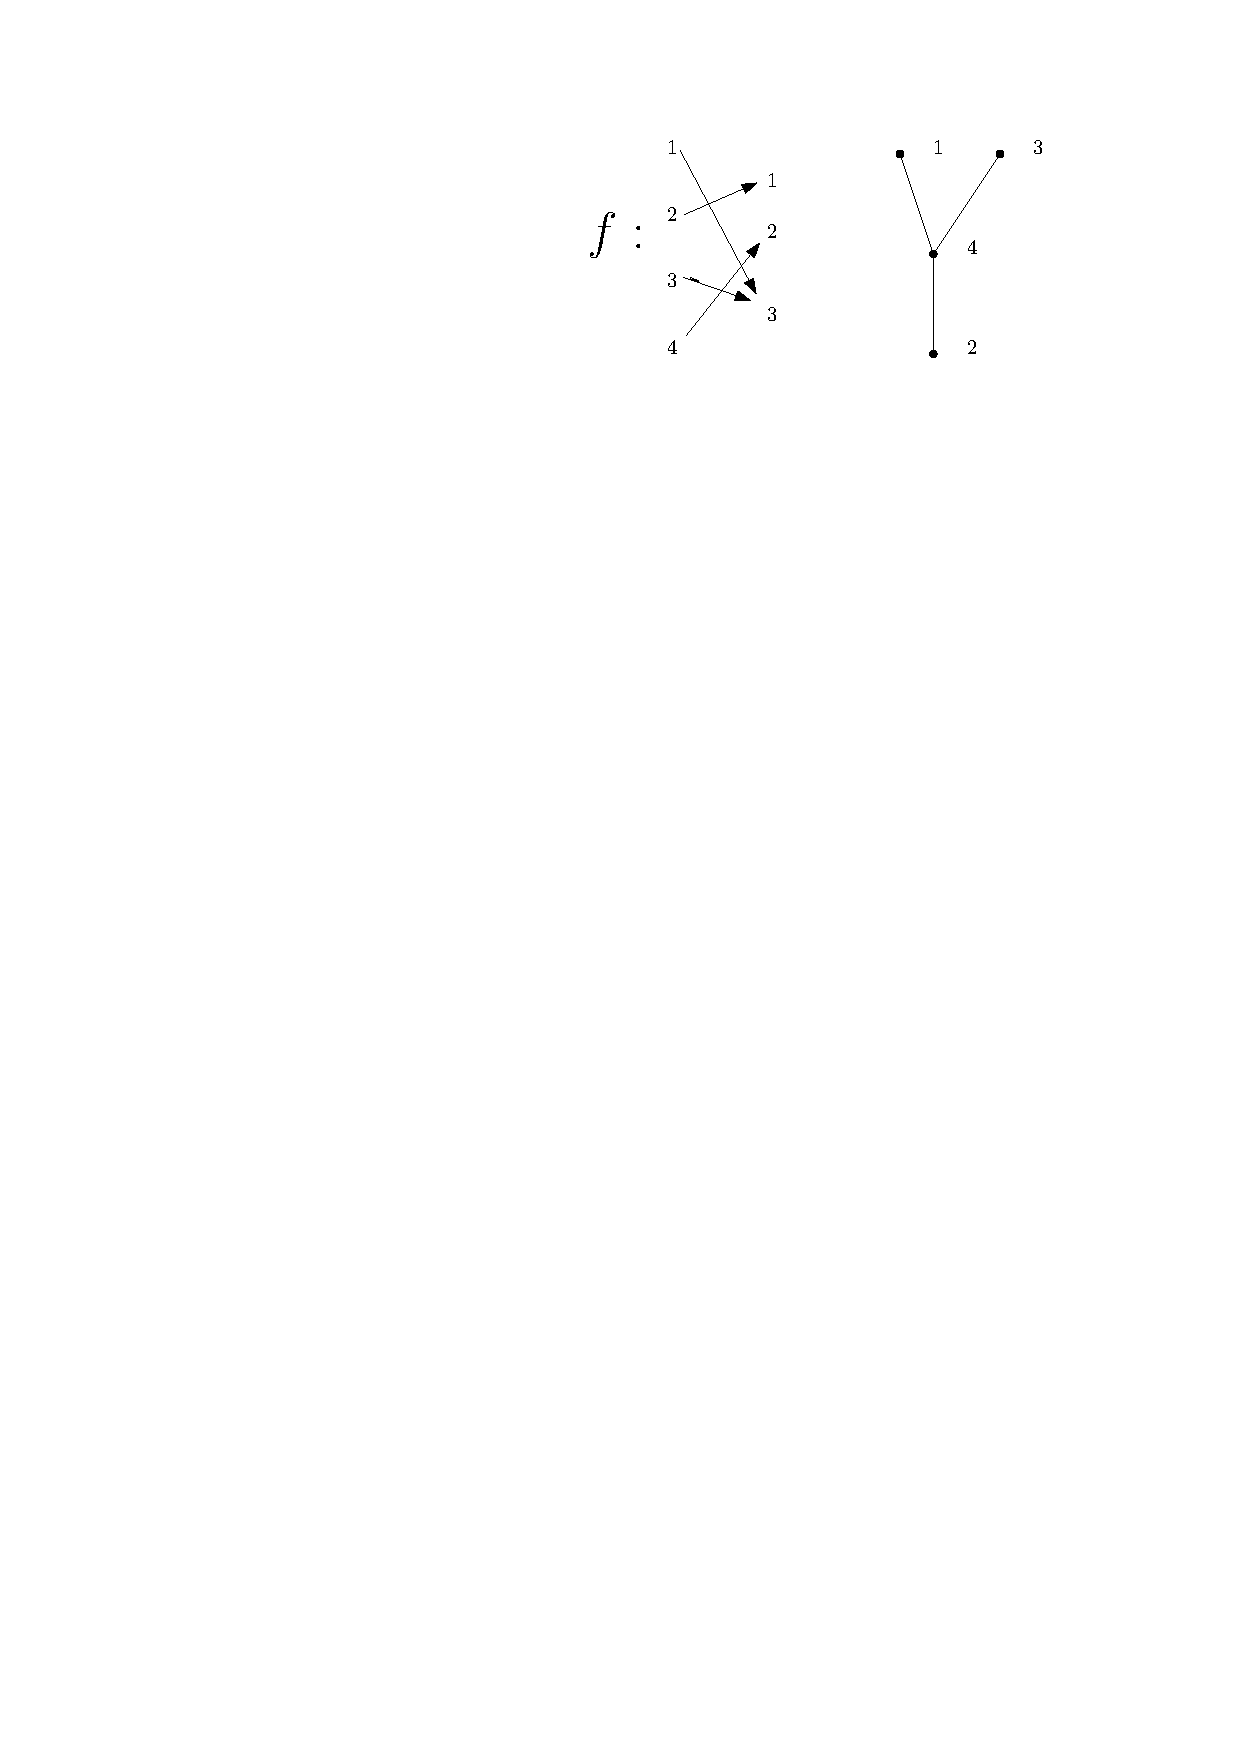
\includegraphics[scale=1]{images/packedWordOrder.pdf}
	\caption{The Hasse diagram of the linear order inherited by the map $f$. \label{fig:packedWordOrder}}
\end{figure}

For instance, if $f = \{ 1\mapsto 3, 2\mapsto 1, 3\mapsto 3, 4\mapsto 2\}$ is a surjective map $[4]\to[3]$, the inherited order is $\{2 < 4 < \{1, 3  \}\}$ and has rank three.
Its Hasse diagram is presented in \cref{fig:packedWordOrder}.
In this way, a packed word $\mathfrak{p}$ on $I$ is a pair of orders $(\leq_P, \leq_V)$ where $\leq_P$ is a total order in $I$, and $\leq_V$ is a linear partial order on $I$.
In particular, note that any permutation on $I$ can be seen as a packed word on $I$, as any total order is a partial linear order.
This relates to the usual notion of packed words as a word in $[m]$ in the following way:
if we order the elements of $I = \{a_1 \leq_P \dots \leq_P a_k \}$, then the corresponding packed word is 
$$rk_{\leq_V}(a_1)rk_{\leq_V}(a_2) \dots rk_{\leq_V}(a_k) \, .$$

Conversely, for any packed word $\omega = p_1\dots p_k$, there are several pairs of orders $(\leq_P, \leq_V)$ that correspond to the word $\omega $, all of which are isomorphic.

\

Consider for instance the packed words $\omega_1 = 13123$ and $\omega_2 = 32413$.
These correspond to packed words on $\{a, b, c, d, e\}$, for instance $\omega_1$ corresponds to $(a > b > c > d > e, \{b, e\} > d > \{a, c\})$ and $\omega_2$ corresponds to $(a > b > c > d > e, c > \{a, e\} >  b > d)$.


If $I \hookrightarrow J$, by restricting the orders on $I$ to orders on $J$ via the injective map $\hookrightarrow $, we obtain a restriction to a packed word on $J$.
The resulting species with restriction structure is denoted by $\mathtt{PWo}$.

\

It will be useful to represent packed words $\omega $ in $I$ as \textbf{rectangle diagrams labeled by $I$}.
This is done in the following way: let $1\leq m \leq |I|$ be the rank of $\omega$, we place the elements of $I$ in an $m \times |I|$ grid so that the elements are placed horizontally according to the $\leq_P$ order, and vertically according to the $\leq_V$ order.
For instance, the packed word $\omega_1 = 13123 = ( d > e > c > a > b, \{b, e\} > \{a\} > \{d, c\})$ in $\{a, b, c, d, e\}$ can be represented as 
\begin{equation}
\begin{array}{|c|c|c|c|c|}
	\hline   & e &   &   & b \\
    \hline   &   &   & a &   \\
    \hline d &   & c &   &   \\
    \hline 
\end{array}\, \, \, .
\end{equation}




In this way, there are $(n!) \times \sum_{m = 1}^n \sFunc(I, [m])$ elements in $\mathtt{PWo}[I]$, where $n = |I|$ and $\sFunc(A, B)$ counts the surjective functions from $A$ to $B$.
Because each packed word $\omega $ has an isomorphism class of size $n!$, we conclude that there are $ \sum_{m = 1}^n \sFunc(I, [m])$ many packed words, which is expected.

\

\label{defin:pwo}
If we consider a packed word $\omega$ on a set $I$, that is, a pair $(\leq_P, \leq_V) $ of orders in $I$, we write $\mathbb{X}(\omega) = I$.
If $f:J \to I $ is an injective map, the preimage of each order $\leq_P, \leq_V$ is well defined.
Furthermore, the preimage of $\leq_P$ is a total order on $J$, whereas the preimage of $\leq_V$ is a linear order on $J$.
Thus, this defines the packed word $\mathtt{PWo}[f](\omega )$.

\

\subsection{Relation between parking functions and labelled Dyck paths}

Let us first recall the definition of a parking function and of  Dyck path.

\begin{defin}[Parking function]
A parking function $\mathfrak{p} = a_1 \dots a_n$ is a sequence of integers in $[n]$ such that, after reordering $a^{(1)} \leq a^{(2)} \leq \dots \leq a^{(n)}$, we have $a^{(i)} \leq i$ for all $i$.
\end{defin}

Examples of parking functions are $12$, $131$ and $3114$.

\begin{defin}[Dyck path]
Given an $n\times n$ square grid, a \textbf{Dyck path} on this square is an edge path that is always above the main diagonal.
It is a classical result that the number of Dyck paths of size $n$ is enumerated by Catalan numbers.
\end{defin}


To describe species on parking functions we need to use the construction of parking functions as labelled Dyck paths (see for instance \cite{Loehr}).
This notion of species with restrictions will recover a notion of patterns in parking functions studied in \cite{adeniran2022pattern}.

\

Specifically, if $I$ is a set of size $n$, we label a Dyck path $\mathcal D$ on an $n\times n$ square grid by a function $f$ that assigns unique values on the set $I$ to each of the \textbf{up} segments of the Dyck path.
If we enrich $I$ with a total order $\prec$ in such a way that in each sequence of \textbf{up} segments, the labels arise in \textbf{increasing} order, Bergeron et.al. construct in \cite{BGLPV2021} a parking function $\mathfrak{p} = \mathfrak{p}(I, \mathcal D, f, \prec) $.
We recover here such construction, adapted to the language presented here, for convenience.

\

There are two steps in this construction.
The first is to realize the labelled Dyck path as a weak set composition $\opi$ of $I$ in $|I|$ parts. The second is to translate the weak set composition $\opi$ and the order $\prec $ in $I$ as a parking function.
We will use an example on $I = \{1, 2, 3, 4, 5\}$ to help us highlight the most important details of this construction, presented in \cref{fig:construction_parking}.
There, we have a Dyck path $\mathcal D$ and a corresponding assignment $f$ to each \textbf{up} segment.
We assume that this labeling set is enriched with the order $1 \prec 2 \prec 3 \prec 4 \prec 5$.

\

\textbf{In the first step} we group each of the labels that occur on the $i$-th vertical line in the $i$-th block of $\opi$.
This gives us a set composition with exactly $n$ parts, of a set with $n$ elements.
Notice as well that it is possible that there are some parts that are empty sets, as it happens in the example given in \cref{fig:construction_parking}.

\textbf{In the second step} we read off the position of each of the labels of $I$, writing down in which part these occur.
Bergeron et. al. proved in \cite{BGLPV2021} that the resulting sequence is a parking function of size $n$.
In the example in \cref{fig:construction_parking}, for instance, we notice that there are no entries in the second block, so $2$ does not occur in the corresponding parking function.
Because there are three elements in the first block, namely $245$, in the parking function $\mathfrak p $ the character $1$ arises three times, on the second, fourth and fifth position.

\begin{figure}
    \centering
    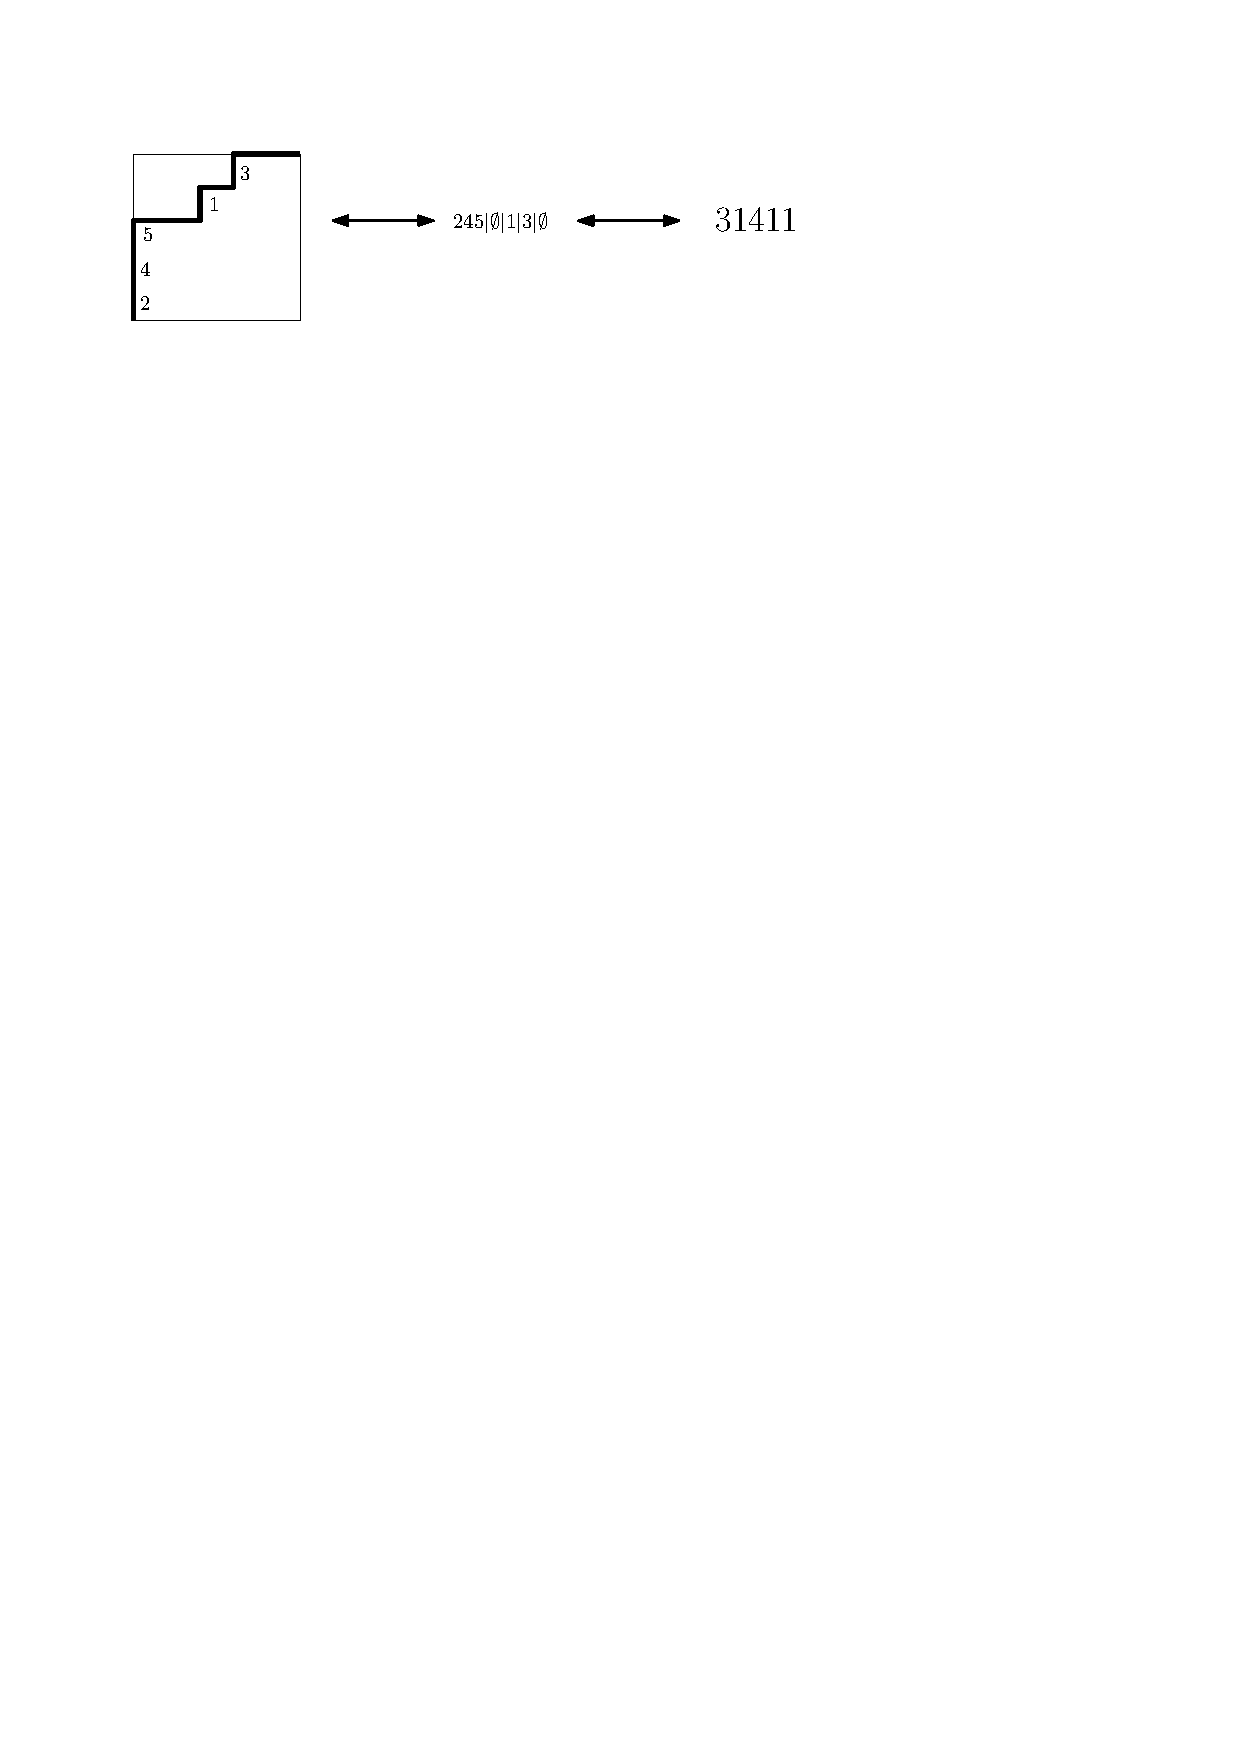
\includegraphics{images/correspondence_parking.pdf}
    \caption{This is an example of a Dyck path labelled by the set $I =\{1, 2, 3, 4, 5\}$. We enrich this set with the usual order on the integers.}
    \label{fig:construction_parking}
\end{figure}


\subsection{Species on parking functions}

This forms the species of \textbf{parking functions}, $\mathtt{PF}$, by letting $\mathtt{PF}[I]$ be the collection of all parking functions $\mathfrak{p} = \mathfrak{p}(I, \mathcal D, f, \prec)$, that is Dyck paths $\mathcal D$ in an $|I|\times |I|$ diagram, labelled by elements of $I$ along with an order $\prec$ of $I$.
We can give it a notion of species with restrictions: for each inclusion $\iota : I \hookrightarrow J $ and a labelled Dyck path $(J, \mathcal D, f, \prec)$ on $J$, the restriction $\mathtt{PF}[\iota](J, \mathcal D, f, \prec) = (I, \mathcal D|_I, f|_I, \prec|_I)$ has an intuitive meaning, except perhaps for
$\mathcal D|_I$, which we clarify in the following.
This is done via a notion of \textbf{tunnels}, introduced by Elizalde in \cite{elizalde2003simple}.
Specifically, the corresponding Dyck path is defined to be the restricted Dyck path by taking the \textbf{tunnels} labelled by elements in $I$, relabelling sequences of \textbf{up} segments if necessary to preserve the increasing property.
One can see in \cref{fig:construction_parking} how this works on the example given above, as well as the corresponding parking function.


\begin{figure}[h]
\centering
    \subfloat[\centering The parking function 31411 and its restriction]{{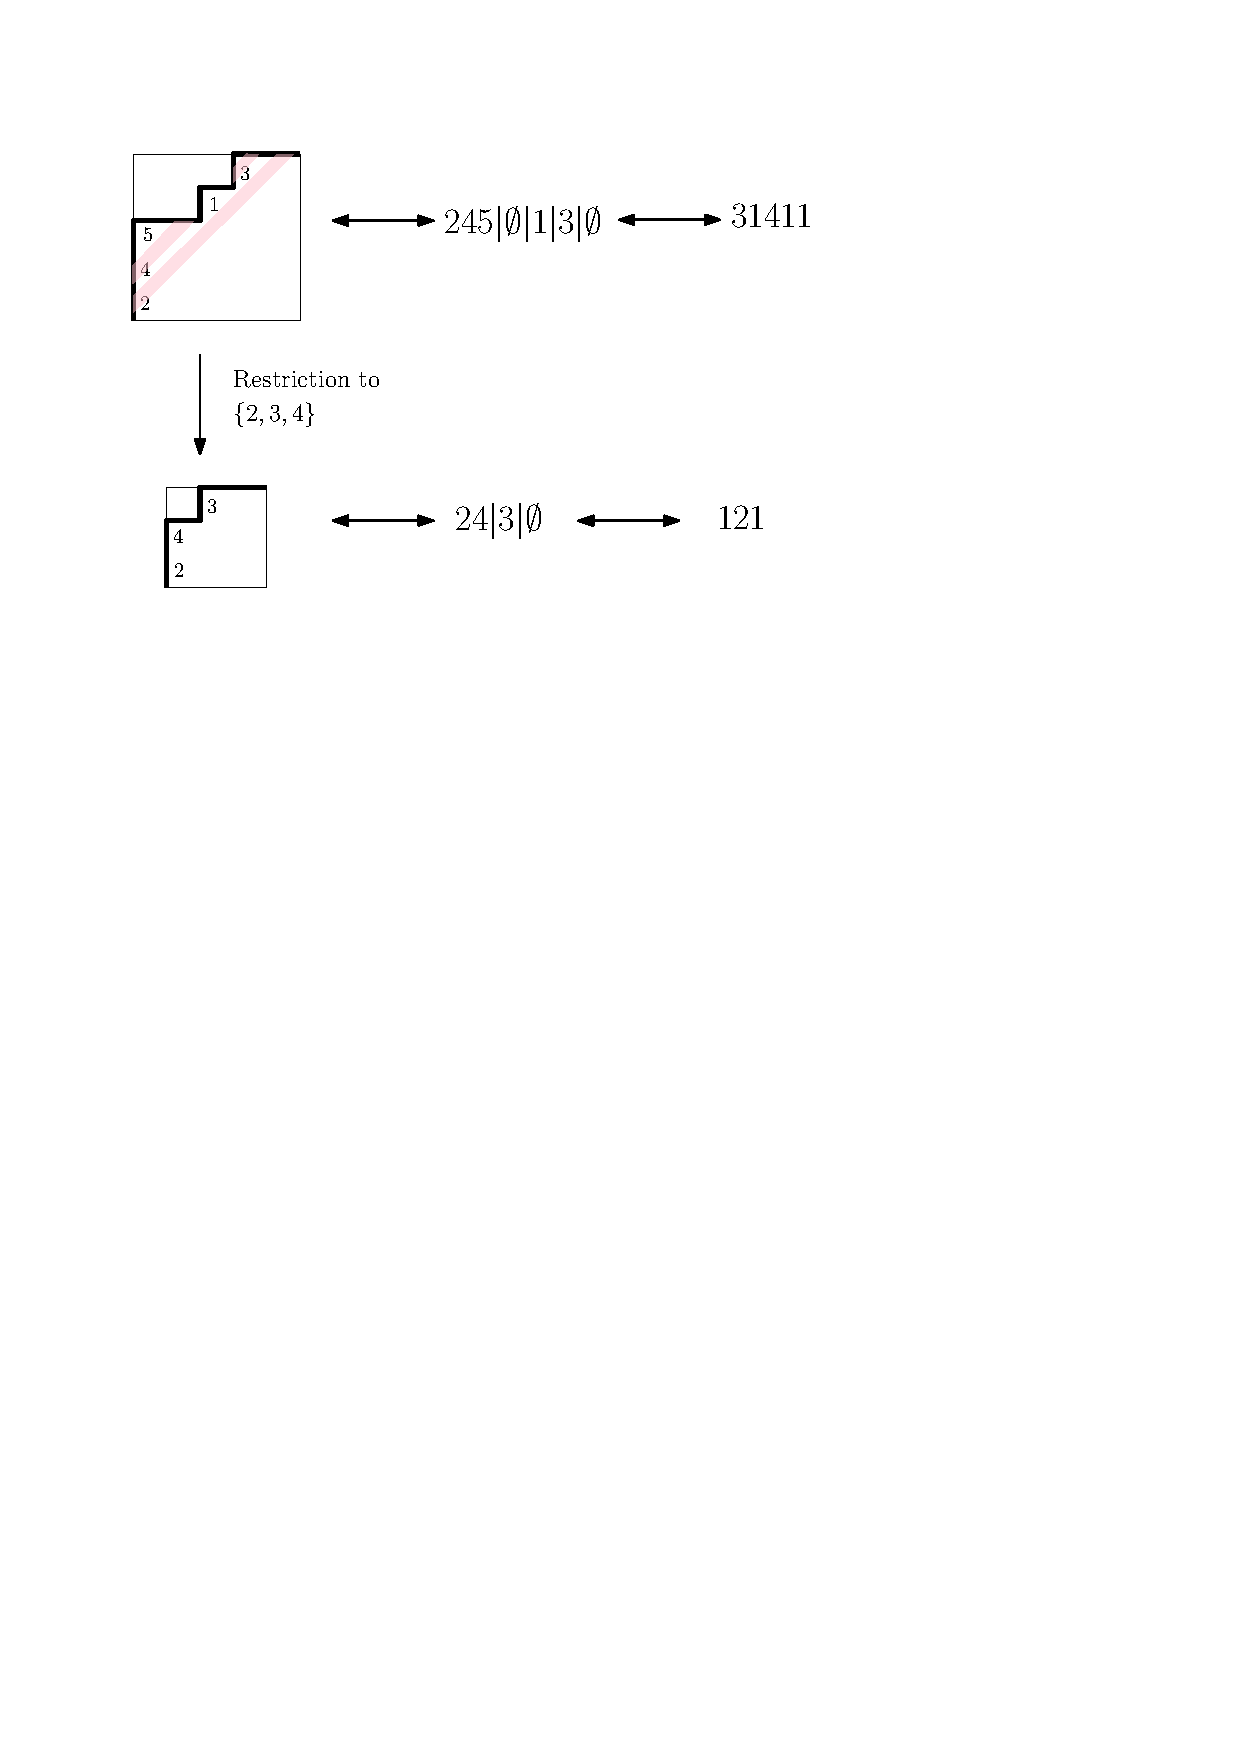
\includegraphics[height=4.8cm]{images/restrictions_parking.pdf} }}%
    \qquad
    \subfloat[\centering The parking function 41511 and its restriction]{{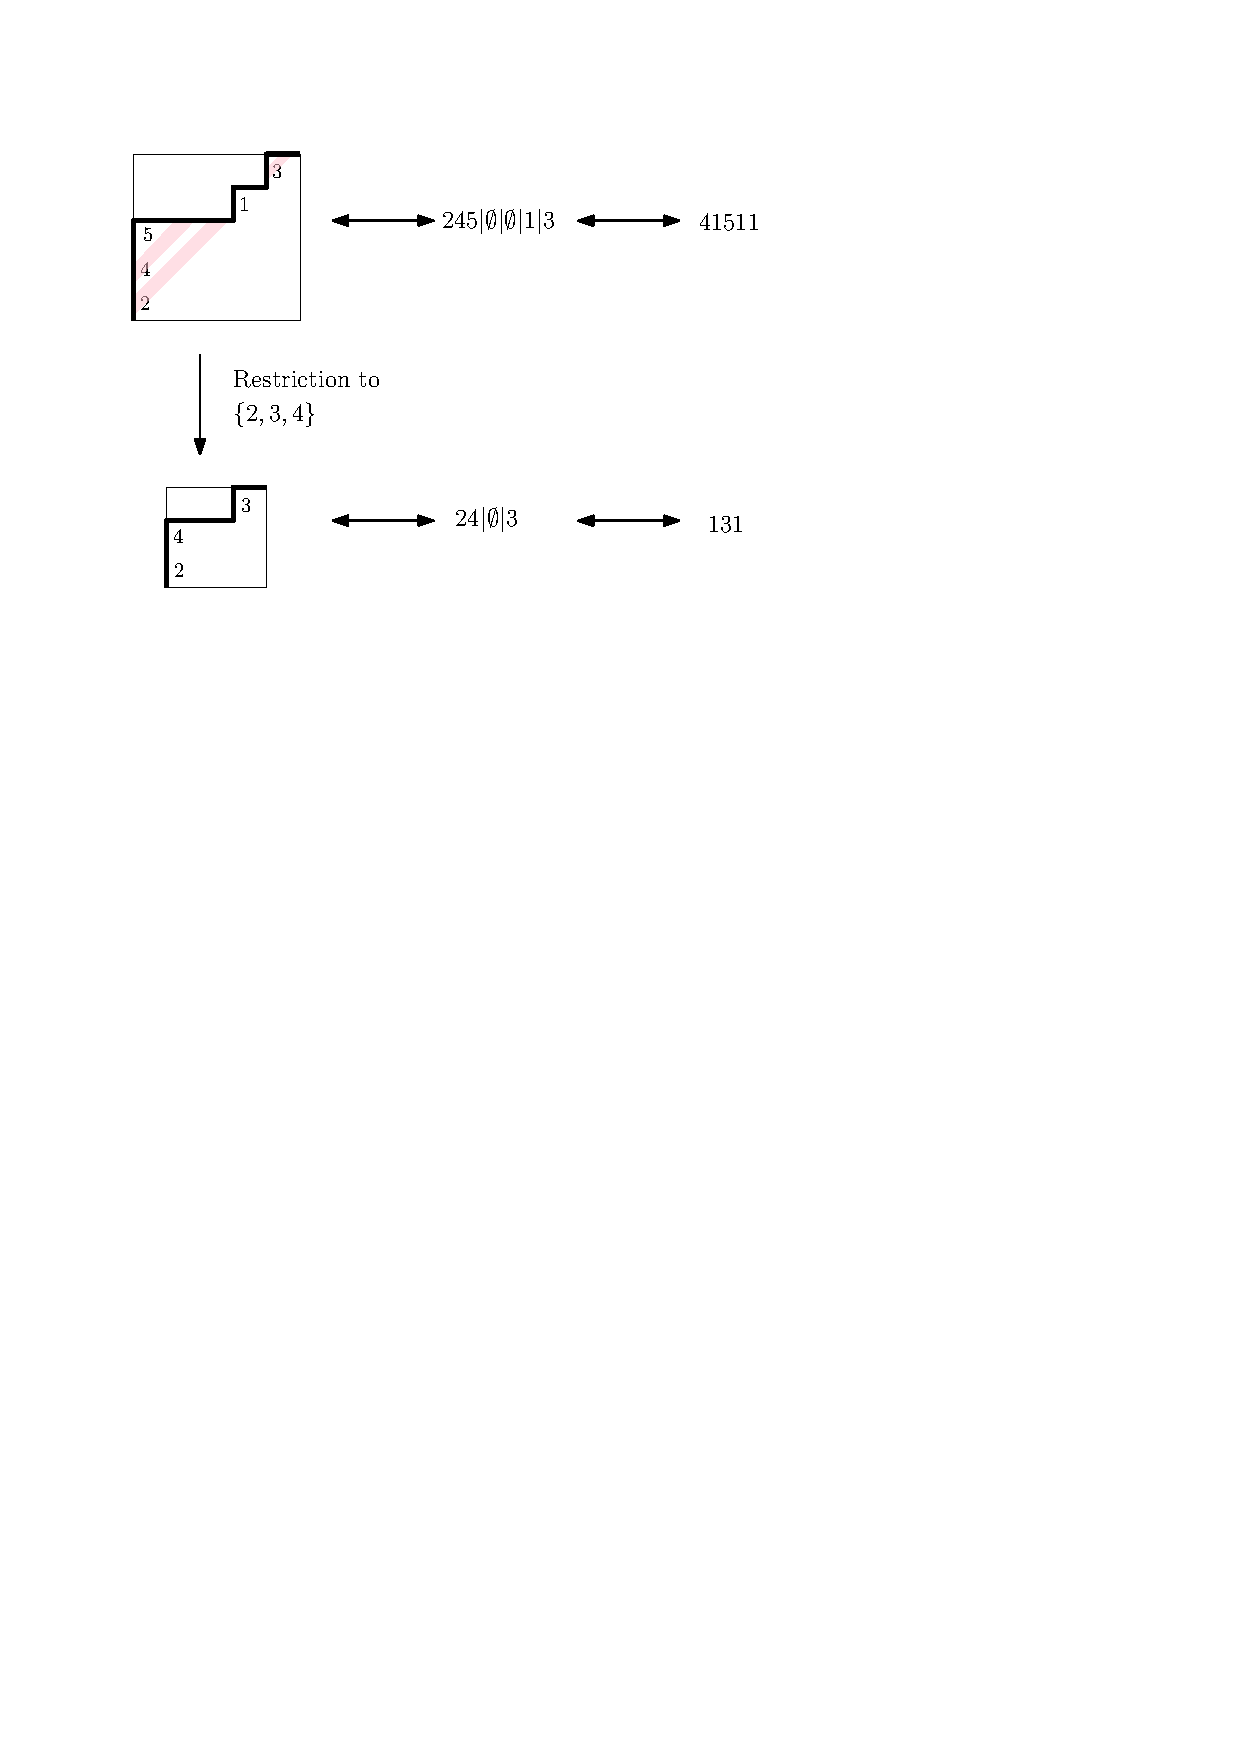
\includegraphics[height=4.8cm]{images/restrictions_parking_other.pdf}}}%
    \caption{\label{fig:restriction_parking}}%
\end{figure}



The following claim is self evident and can be established by the same methods presented in \cite{Penaguiao2020}.

\begin{prop}[Species with restrictions on parking functions]
This forms a species with restrictions structure.
Furthermore, the diagonal sum $\oplus $ endows $\mathtt{PF}$ with a monoid structure, and the resulting Hopf algebra $\mathcal A(\mathtt{PF})$ is free.
\end{prop}

The proof is immediate.
For the last part, we observe that because $\mathtt{PF}$ is NCF (see below in \cref{defin:ncf}), we have from \cite{Vargas} that this algebra is free.

\begin{smpl}
The five smallest parking functions are $\emptyset, 1, 11, 12$ and $21$.
The sixteen parking functions of size three are displayed in \cref{fig:PF3}, along with its corresponding labelled Dyck paths.

For any parking function $\mathfrak p$ of size three, we have $\pat_{\emptyset}(\mathfrak p) = 1$ and $\pat_1(\mathfrak p) = 3$.
The values of $\pat_{11}, \pat{12}$ and $\pat{21}$ in pattern functions of size three are represented below in \cref{tab:PF3}.
There, one can also easily check the relation $\pat_1^2 = \pat_1 + 2(\pat_{11} + \pat_{12} + \pat_{21})$, predicted from \eqref{eq:prodrule}.
\end{smpl}
\begin{table}
\begin{tabular}{ c |  c c c c c c c c c c c c c c c c}
 0  & \small{111} & \small{112} & \small{121} & \small{211} & \small{113} & \small{131} & \small{311} & \small{122} & \small{212} & \small{221} & \small{123} & \small{132} & \small{213} & \small{312} & \small{231} & \small{321}\\ 
 11 & 3 & 2 & 2 & 2 & 1 & 1 & 1 & 1 & 1 & 1 & 0 & 0 & 0 & 0 & 0 & 0 \\  
 12 & 0 & 1 & 0 & 0 & 2 & 1 & 0 & 2 & 1 & 0 & 3 & 2 & 2 & 1 & 1 & 0 \\  
 21 & 0 & 0 & 1 & 1 & 0 & 1 & 2 & 0 & 1 & 2 & 0 & 1 & 1 & 2 & 2 & 3 \end{tabular}
\caption{\label{tab:PF3}Pattern functions evaluated at parking functions of length three.}
\end{table}

\begin{figure}
\centering
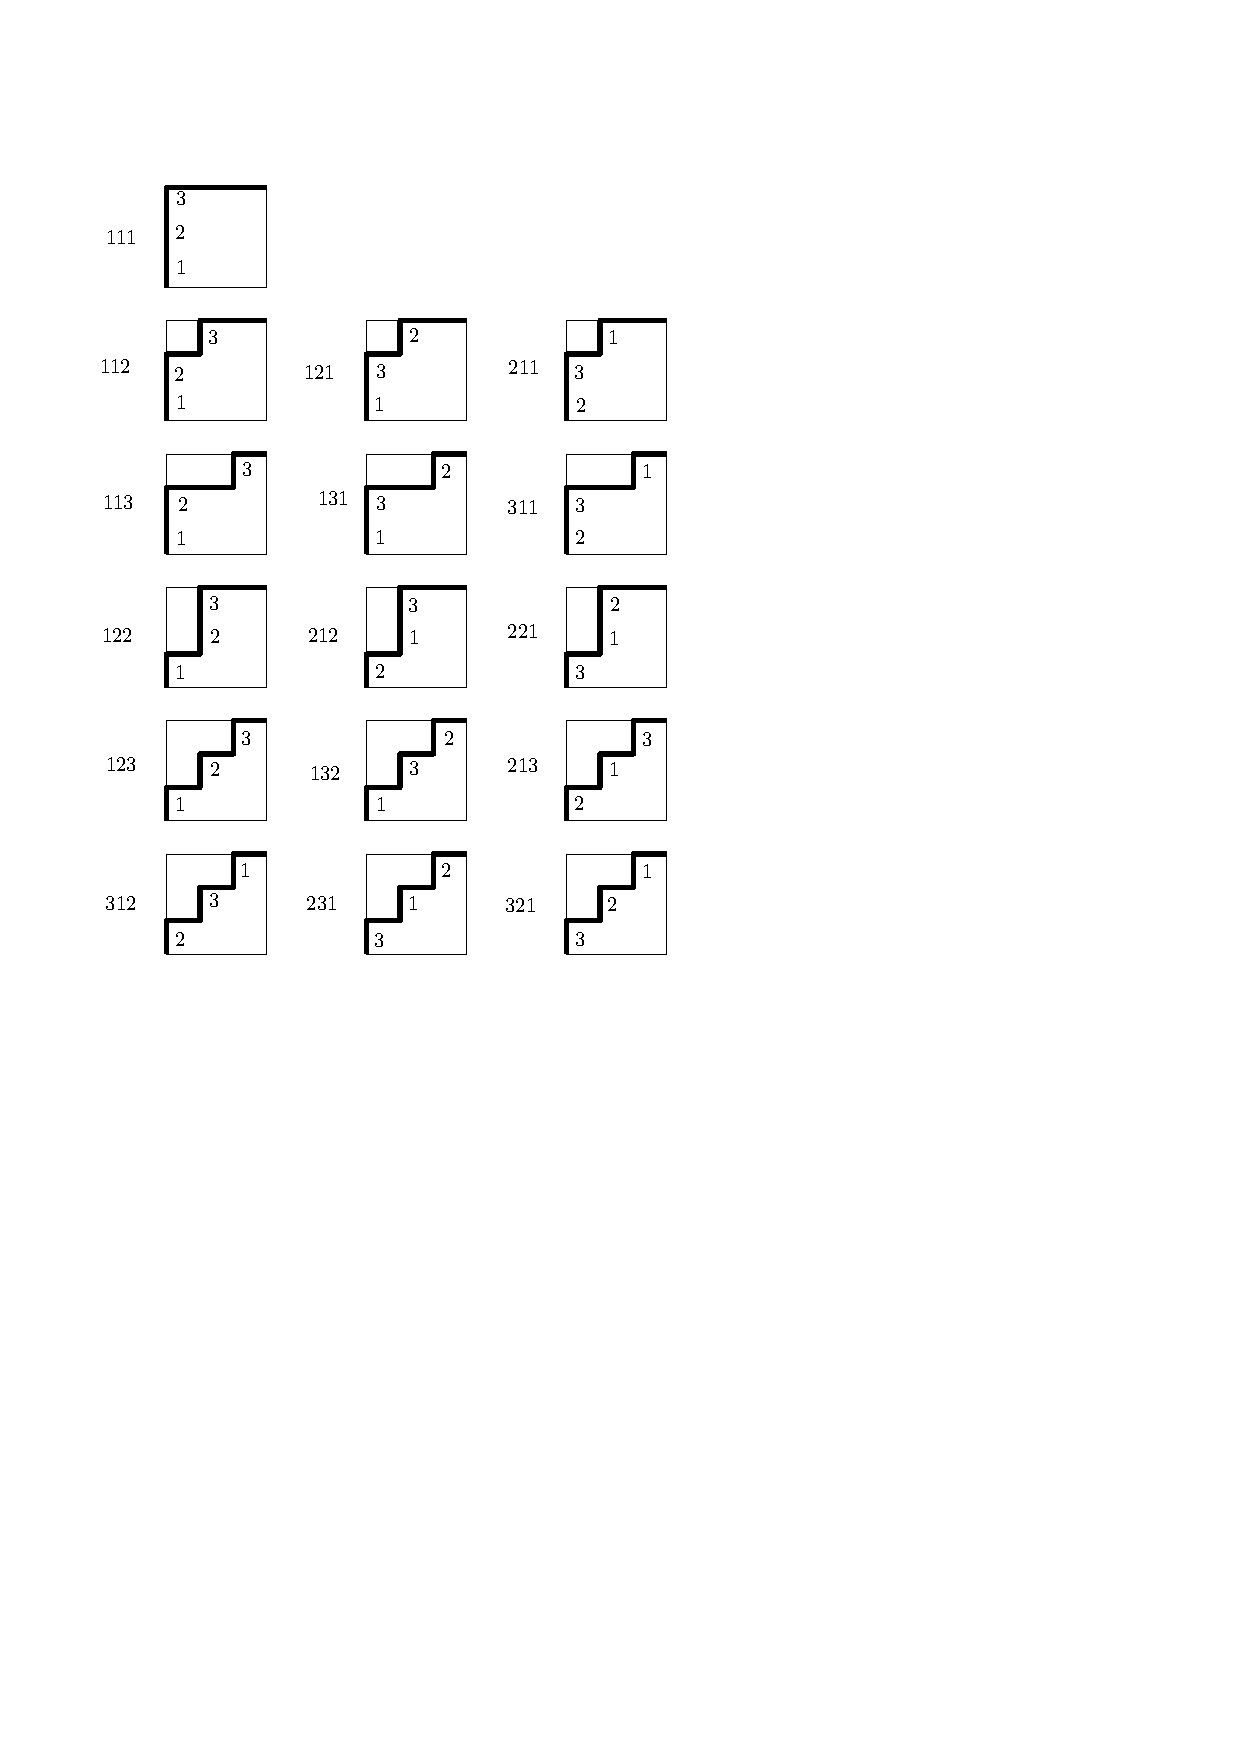
\includegraphics[scale=1]{images/parking_functions_3}
\caption{\label{fig:PF3}}
\end{figure}





\

\section{The antipode formula for the pattern algebras \label{sec:formula_general}}
\

In this section we give a general formula for the antipode of a pattern algebra, whenever our connected species with restrictions is of the form $L \times \mathtt{h}$. This antipode formula is a dual analogue of the antipode formula in \cite{BergeronBenedetti}, where a similar formula was obtained for linearized Hopf species.

\

The formula obtained is not cancellation free, but it servers as a starting platform to explore the cancellation free formulas for the cases presented above: permutations, packed words and parking functions. The requirement that our species with restrictions is divisible by $L$ explains why no cancellation free formulas for other species with restrictions, for instance in marked permutations, introduced in \cite{Penaguiao2020}, were found.

\

We start by recalling Takeuchi's formula, from above in \cref{lm:takeuchi}.
If $H = (H, \mu, \iota, \Delta, \epsilon, S)$ is a Hopf algebra such that $(  \iota  \circ\epsilon - \id_H)$ is $\star$-nilpotent, then 
$$S = \sum_{k\geq 0 }  ( \iota  \circ\epsilon- \id_H)^{\star k}\, . $$

Recall that for a filtered Hopf algebra $H$, and so for any pattern Hopf algebra $\mathcal A (\mathtt{h})$, $(\epsilon\circ \iota - \id_H)$ is $\star$-nilpotent. 

\

\subsection{$L\times -$ species with restrictions}


In \cite[Corollary 3.4.]{Penaguiao2020} it was shown that in species with restrictions $\mathtt{h}$, any factorization into $\ast$-indecomposibles is unique up to order.
In some species with restrictions, we can also drop the ``up to order'' adjective, as there is exactly one factorization into $\ast$-indecomposibles full stop. We precise this in the following definition.
Before that, we want to precise our notation.
We will be using $\star$ for the operation on $\End (H)$ and we will be using $\ast $ for the associative structure on a species.



\begin{defin}[Non-Commuting Factorization on pattern Hopf algebras]\label{defin:ncf}
A monoidal species with restrictions is called a \textbf{non-commuting factorization} species, or simply an NCF species, if any element $x$ has a unique factorization into $\ast$-indecomposibles elements $x = x_1 \ast \dots \ast x_n$.
\end{defin}


\begin{lm}[Linear species with restrictions have NCF]
Let $\mathtt{h}$ be a connected species with restrictions.
Then $L \times \mathtt{h}$ has NCF.
\end{lm}

\begin{proof}
Let $x = x_1 \ast \dots \ast x_k $ and $ y =  y_1 \ast \dots \ast y_n$ such that $x \sim y$.
From \cite[Corollary 3.4.]{Penaguiao2020}, we know that $k = n$ and the multisets $\{x_i\}_{i=1}^k,  \{y_i\}_{i=1}^n$ are the same.
It remains to show that the factorizations order coincide and that we have $x_i \sim y_i$ for $i = 1, \dots , n$.
To that effect we act by induction, where $n = 1$ is trivial.

%\

%For the induction step, let us consider the bijection $\sigma:[n] \to [n]$ such that $y_{\sigma(i)} \sim x_i$ given by \cite[Corollary 3.4.]{Penaguiao2020}.
We write $x_i = (l_i, p_i)\in (L\times \mathtt{h})[I_i]$ and $y_i = (m_i, q_i)\in (L\times \mathtt{h})[J_i]$.
Finally, write $x = (l, p) \in (L\times \mathtt{h})[I] $ and $y = (m, q) \in (L\times \mathtt{h})[J]$.
By hypothesis, we have that $x \sim y$, so there exists some bijection $\phi: J \to I$ such that $ (L\times \mathtt{h})[\phi](x) = y$.
This bijection yields a correspondence between two linear orders $L [\phi] (l_1 \ast \dots \ast l_n) = m_1\ast \dots \ast m_n $.
Observe that $I_1$ and $J_1$ are ideals in $l1\ast \dots \ast l_n$ and $m_1 \ast \dots \ast m_n$, respectively, as seen in \cref{prop:linorderideals}.
So either $\phi (I_1)= J_1 $ or $\phi (I_1)\supsetneq J_1 $.
Assume wlog that $|I_1 | \geq	 |J_1|$ and assume for sake of contradiction that $|I_1| > |J_1|$, and consider the following factorization of $x_1 $:
\begin{equation}\label{eq:linearpats:non_trivial_fact}
x_1 = x|_{I_1} \sim y|_{\phi(I_1)} = y_1|_{\phi(I_1) \cap J_1} \ast (y_2 \ast \dots \ast y_n)|_{(J\setminus J_1) \cap \phi(I_1)}\, . 
\end{equation}

Now, because $|I_1| > |J_1|$ and that $\phi $ is a bijection, we have that $| (J\setminus J_1) | + | \phi(I_1) | = n - |J_1| + |I_1| > n$, so the intersection $(J\setminus J_1) \cap \phi(I_1)$ is non-empty.
on the other hand, $\phi(I_1) \cap J_1 = J_1$.

Going back to \eqref{eq:linearpats:non_trivial_fact}, we get a non-trivial factorization of $x_1$, which contradicts the fact that we started with a factorization into indecomposibles.

This is a contradiction, thus $|I_1 | = |J_1|$, which shows that $\phi(I_1) = J_1$.
Therefore,  $\phi(I\setminus I_1) = J \setminus  J_1$, $ \mathtt{h}[\phi] (p|_{I_1}) = q|_{J_1} $ and $ \mathtt{h}[\phi] (p|_{I \setminus I_1}) = q|_{J \setminus J_1} $.

\

In conclusion, we get that $x_1 \sim y_1$ and $x_2 \ast \cdots \ast x_n \sim y_2 \ast \cdots \ast y_n$, via $\phi$.
By induction hypothesis, this tells us that $x_2 \sim y_2, \cdots , x_n \sim y_n$, as desired.
\end{proof}


\begin{cor}
If $\mathtt{h} = \mathtt{L} \times \mathtt{h}'$, then $\mathcal A(\mathtt{h})$ is free.
\end{cor}
This follows from \cite{Vargas}, after we recognize that $\mathtt{L} \times \mathtt{h}'$ has NCF.

\

The pattern Hopf algebra on permutations, on packed words and on parking functions all satisfy the NCF property.
In fact, permutations, packed words and parking functions are of the form $\mathtt{L} \times \mathtt{h}$.
This property allows for an easy manipulation of the coproduct, and results in a more tractable approach to the antipode formula.

\begin{defin}[Composition poset and cumulative sum]
Recall that we write $\mathcal C_n$ for the set of compositions of size $n$.
We will define $\mathbf{CS}$, a bijection between $\mathcal C_n $ and $2^{[n-1]}$, as follows.
If $\alpha =(\alpha_1, \dots, \alpha_{\ell} ) \in \mathcal C_n$, define $f_i = \sum_{j=1}^i$ and 
$$\mathbf{CS}(\alpha) = \{f_i | i = 1, \dots, \ell - 1\} \, .$$

This bijection allows us to define an order $\leq $ in $\mathcal C_n$, via the pullback from the boolean poset in $2^{[n-1]}$.
This order can be defined as well as follows: we say that $\alpha \leq \beta$ if $\alpha$ arises from $\beta $ after merging and adding consecutive entries.
\end{defin}

\
Recall that a QSS $\III = (I_1, \dots , I_n)$ of $y\in L\times \mathtt{h}[I]$ from $x_1, \dots, x_n$ satisfies $y|_{I_i} = x_i$ for all $i = 1, \dots , n$, and $I = \bigcup_i I_i$.

\begin{defin}[Compositions and QSS]
Let $x \in (L\times \mathtt{h})[J], y \in (L\times \mathtt{h})[I]$, and $x = x_1\ast \dots \ast x_n$ be the unique factorization of $x$ into indecomposibles.
Further say that $y = (<_y, \iota)$, where $<_y$ is a linear order in $I$.
Let $\III = (I_1, \dots , I_n)$ be a QSS of $y$ from $x_1, \dots, x_n$ and consider a composition $\alpha \models n$.

\

Suppose that $ \mathbf{CS} (\alpha) = \{f_1, \dots, f_{\ell(\alpha) - 1} \}$ and use the convention that $f_0 = 0$ and $f_{\ell(\alpha)} = n$. 
Then we define for $i = 1, \dots, \ell(\alpha)$:
\[I^{\alpha}_i := I_{f_{i-1} + 1} \cup \dots \cup I_{f_i} \quad , \quad x^{\alpha}_i := x_{f_{i-1} + 1} \ast \dots \ast x_{f_i}.\]

\

Two indices $i< j$ are said to be \textbf{merged} by $\alpha$ if there is some $k$ in $\{1, \dots, n\}$ such that $ f_{k-1} < i < j \leq f_k$.
We say that a QSS $\III$ of $y$ from $x_1, \dots , x_n$ is $\alpha $-stable if $(I^{\alpha}_i)_i \text{ is a QSS of $y$ from } (x^{\alpha}_i)_i$ and, whenever $x_i \sim x_j$ and $i < j$ are merged with $\alpha $, then $I_i <_y I_j$ with respect to the linear order $m$.

\

Finally, we define 
$$\mathcal I^{x, y}_{\III} \coloneqq \left\{ \alpha \models n \Big| \III \text{ is an $\alpha$-stable QSS of $y$ from } (x_i)_i \right\} \, .$$

\end{defin}

\

\begin{smpl}[$\alpha$-stable QSS on $\mathtt{PWo}$]
Consider the packed word $\omega = 21 \oplus 111 = 21333 = (1 < 2 < 3 < 4 < 5, 2 < 1 < \{3, 4, 5\})$ on the set $[5]$.
This packed word has three QSS from $21, 1, 11$, precisely $\III_1 =(12, 3, 45)$, $\III_2 =(12, 4, 35)$ and $\III_3 =(12, 5, 34)$.
All three are $(1, 1, 1)$-stable.

We now observe that $\III_1, \III_2$ and $\III_3$ are $(2, 1)$-stable, but neither $(1, 2)$-stable nor $(3)$-stable.
Indeed, $\III_1^{(1, 2)} = \III_2^{(1, 2)} = \III_3^{(1, 2)} = (12, 345)$, and $\omega|_{345} = 111$ is not $\omega|_{I_2} \oplus \omega|_{I_3}$ for any of the QSS.
On the other hand, $\III_1^{(2, 1)} = (123, 45)$, $\III_2^{(2, 1)} = (124, 35)$ and $\III_3^{(2, 1)} = (125, 34)$, in each case is easy to note that $\omega|_{I_1^{(2, 1)}} = 21\oplus 1$ and $\omega|_{I_2^{(2, 1)}} = 11$ for each of the QSS.

Therefore, in each case we get
$$\mathcal I_{\III}^{21\oplus 1\oplus 11, 21333} = \{(1, 1, 1), (2, 1)\}\, . $$
\end{smpl}


The following example portrays the significance of adding the additional requirement that $I_i < I_j$ whenever $x_i \sim x_j$ and $i, j$ are merged by $\alpha$, in the context of packed words.

\begin{smpl}[$\alpha$-stable when $x_i \sim x_j$]
\raul{belabour example, on the notes from Raul}
$\omega =2133$ with QSS $(13, 2, 4)$ and $(13, 4, 2)$, these are QSS of $\omega $ from $ 12, 1, 1$.
First is $(1, 2)$-stable, whereas second is not $(1, 2)$-stable.
\end{smpl}


A simple method to check when a given QSS is $ælpha$-stable is the following.

\begin{obs}\label{obs:pwords-characterisation}
In general, it is easy to see that $\III $ is $(\underbrace{1, \dots , 1}_\text{$i-1$ times}, 2, 1, \dots, 1)$-stable if and only if $I_i < I_{i+1}$ on both orders of $\omega$.
\end{obs}

\


\begin{obs}
Let $\mathtt{h}$ be a species with restrictions, $y, x_1, \dots, x_n \in \mathcal G(\mathtt{h})$ and $\III$ a QSS of $y$ from $x_1\dots, x_n$.
Call $x \coloneqq x_1 \ast \dots \ast x_n$.
Then, $\mathcal I^{x, y}_{\III}$ has a unique maximal element, $\mathbb{1}$.
\end{obs}

The following is the main theorem in this section

\begin{thm}\label{thm:general_antipode}
For a species with restrictions $\mathtt{h}$ that is a multiple of $\mathtt{L}$, and an element $x$, along with its factorization $x=x_1 \ast \dots \ast x_n$, we have the following antipode formula in $\mathcal A (\mathtt{h})$:

$$S(\pat_x) = \sum_y \pat_y \sum_{\substack{\III \text{ QSS of $y$}\\ \text{from }x_1, \dots , x_n}}  \sum_{\alpha \in \mathcal I^{x, y}_{\III}} (-1)^{\ell ( \alpha)} \, .$$
\end{thm}

\begin{proof}
\begin{align*}
\Delta^{\circ (k-1)} (\pat_x)
    =& \sum_{x = \chi_1 \ast \dots \ast \chi_k} \pat_{\chi_1}\otimes \dots \otimes \pat_{\chi_k}
\end{align*}
Because the species with restrictions $\mathtt{h}$ has NCF, the only ways to factorize $x$ into $k$ factors is to start from the original factorization $x = x_1 \ast \dots \ast x_n$ and bracket these factors, possibly empty, into $k$ blocks.
Therefore, we can enumerate these factorizations using weak compositions, as follows:

\begin{align*}
(\iota \circ \epsilon -  \id_{\mathcal A (\mathtt{h})})^{\star k} (\pat_x)
    =& (-1)^k  \mu^{\circ(k-1)}( \id_{\mathcal A (\mathtt{h})} - \iota \circ \epsilon)^{\otimes k} \Delta^{\circ(k-1)} (\pat_x)\\
    =& (-1)^k  \mu^{\circ(k-1)}( \id_{\mathcal A (\mathtt{h})} - \iota \circ \epsilon)^{\otimes k}\left(\sum_{\substack{\alpha\models^0 n \\ \ell(\alpha) = k}} \pat_{x^{\alpha}_1} \otimes \dots \otimes \pat_{x^{\alpha}_k} \right) \\
    =&  (-1)^k  \mu^{\circ(k-1)} \sum_{\substack{\alpha\models n \\ \ell(\alpha) = k}}  \pat_{x^{\alpha}_1} \otimes \dots \otimes \pat_{x^{\alpha}_k}\\
    =&  (-1)^k \sum_{\substack{\alpha\models n \\ \ell(\alpha) = k}}  \pat_{x^{\alpha}_1}  \cdots \pat_{x^{\alpha}_k}
\end{align*}

Note how we used that $(\id_{\mathcal A (\mathtt{h})} - \iota \circ \epsilon ) (\pat_x) = \mathbb{1}[x \neq 1]\pat_x$.
Thus, the theorem follows from Takeuchi's formula (\cref{lm:takeuchi}) after some clever rearrangements:

\begin{align*}
S(\pat_x)&= \sum_{k\geq 0 } (\iota \circ \epsilon -  \id_{\mathcal A (\mathtt{h})})^{\star k} (\pat_x) \\
         &= \sum_{\alpha \models n} (-1)^{\ell(\alpha)} \pat_{x^{\alpha}_1} \cdots \pat_{x^{\alpha}_{\ell(\alpha)}}\\
         &= \sum_{\alpha \models n } (-1)^{\ell(\alpha)} \sum_y \pat_y \binom{y}{x^{\alpha}_1,  \dots , x^{\alpha}_{\ell(\alpha)}}\\
         &= \sum_y \pat_y \sum_{\alpha \models n} \sum_{  \substack{\III \text{ QSS of $y$}\\ \text{from }x^{\alpha}_1,  \dots , x^{\alpha}_{\ell(\alpha)} }} (-1)^{\ell(\alpha)}\\
         &= \sum_y \pat_y \sum_{  \substack{\III \text{ QSS of $y$}\\ \text{from }x_1 , \dots ,  x_n }} \sum_{\alpha \in \mathcal I^{x, y}_{\III}} (-1)^{\ell(\alpha)}.
\end{align*}

All equalities but the last one are simple rearrangements.
To motivate the last equality, we will construct a series of bijections, for each composition $\alpha \models n$:
\begin{align*}
    \Phi_{\alpha}^{x, y} = \Phi_{\alpha} : \left\{ \JJJ \text{ QSS of $y$ from $x^{\alpha}_1, \dots, x^{\alpha}_{\ell(\alpha)}$}\right\} &\to \left\{ \III \text{ $\alpha$-stable QSS of $y$ from $x_1, \dots, x_n$}\right\}\, , \\
    (J_1, \dots, J_{\ell(\alpha)} ) &\mapsto (I_1, \dots , I_n).
\end{align*}

\

Recall that $y = (<_y, \iota)$ induces a linear order $m$ in $I$.
The sets $(I_i)_i$ are defined so that $J_s = I_{f_{s-1}+1} \uplus \dots \uplus I_{f_s}$, that $|I_i | = |x_i|$ and that $I_i <_y I_j $ whenever $f_{s-1} < i < j \leq f_{s}$.
This is easily seen to be an $\alpha$-stable QSS of $y$ from $x_1, \dots, x_n$.

\

Inversely, we define:
\begin{align*}
    \Psi_{\alpha}^{x, y} = \Psi_{\alpha}  : \left\{ \III \text{ $\alpha$-stable QSS of $y$ from $x_1, \dots, x_n$}\right\} &\to \left\{ \JJJ \text{ QSS of $y$ from $x^{\alpha}_1, \dots, x^{\alpha}_{\ell(\alpha)}$}\right\} \, , \\
    (I_1, \dots , I_n) &\mapsto (I_1^{\alpha}, \dots, I^{\alpha}_{\ell(\alpha)} ),
\end{align*}
where we recall that $I^{\alpha}_i = I_{f_{s-1}+1} \cup \dots  \cup I_{f_s}$.

\

The maps $\Psi_{\alpha}$ and $\Phi_{\alpha}$ are easily seen to be inverses of each other, establishing the bijection and the desired result.
\end{proof}

\

%\begin{smpl}[Example in permutation patterns]
%Consider $\sigma = 312$ and $\pi = 123 = 1\oplus 1 \oplus 1$.
%We will compute the antipode of $\pat_{\sigma}$ using this formula, by computing $\mathcal I^{\sigma, \pi}_{\III}$ for each QSS $\III$.
%
%\end{smpl}

\begin{prop}[Filtered structure of $\mathcal I$]\label{prop:filter_structure_I}
For a species with restrictions $\mathtt{h}$ that is a multiple of $\mathtt{L}$, and an elements $x\in  \mathtt{h}[J], y\in \mathtt{h}[I]$, along with a factorization into $\ast$-indecomposibles $x = x_1 \ast \dots \ast x_n$ and a QSS $\III$ of $y$ from $x_1, \dots, x_n$, we have that $\mathcal I^{ x, y}_{\III}$ is a filter.
That is, if $\alpha \in \mathcal I^{ x, y}_{\III}$ and $\beta \geq \alpha$ then $\beta \in \mathcal I^{ x, y}_{\III}$.

\
Furthermore, if $\mathcal I^{ x, y}_{\III}$ has a unique minimal element distinct from $\mathbb{1}$, then
$$\sum_{\alpha \in \mathcal I^{x, y}_{\III}} (-1)^{\ell(\alpha)} = 0 \, .$$
\end{prop}

\begin{proof}
To establish the first fact, assume that $\alpha \in \mathcal I^{x, y}_{\III}$ and let $\beta \geq \alpha $.
Because $\beta \geq \alpha$, if $\beta $ merges $i < j$ then $\alpha $ merges $i < j$, thus we have that $I_i < I_j$ with respect to the order of $y$.
It remains then to show that $(I^{\beta}_i)_i$ is a QSS of $y$ from $(x^{\beta}_i )_i$, or equivalent that $y|_{I_i^{\beta}} \sim x_i^{\beta}$.

\

However, because $\beta \geq \alpha$, for each $i$ we have $I^{\beta}_i \subseteq I^{\alpha}_j$ so 
\[y|_{I^{\beta}_i} = {\Big(}y|_{I^{\alpha}_j}{\Big )}|_{I^{\beta}_i} =x^{\alpha}_j |_{I^{\beta}_i} = x^{\beta}_i \, .\]

\

For the concluding part, we simply observe that if $\mathcal I^{x, y}_{\III}$ has a unique minimal element $\mathbb{0}$, then it is the interval of a boolean poset $\mathcal I^{x, y}_{\III} = [\mathbb{0}, \mathbb{1}]$.
Furthermore, we have that $\mathbb{0} \neq \mathbb{1}$.
Let $\mathcal K $ be the collection of sets $A \subseteq [n-1]$ that contain $X \coloneqq \mathbf{CS}(\mathbb{0})$.

Consider $\zeta: \mathcal K \to \mathcal K$.
Choose $\chi \in [n-1] \setminus X$, if $X \neq [n-1]$, and define $\zeta (A) = A \Delta \{ \chi \}$.
If no such $\chi $ exists, define $\zeta(A) = A$.
This is an involution on subsets of $[n-1]$ that contain $X$, which corresponds to an involution in compositions in $[\mathbb{0} , \mathbb{1}]$.
It can be seen that this is indeed sign-reversing, so we conclude that 
$$\sum_{\alpha \in \mathcal I^{x, y}_{\III}} (-1)^{\ell(\alpha)} =  \mathbb{1}[[n-1] \setminus X \text{ is empty } ] = \mathbb{1}[\mathbb{1} = \mathbb{0}] \, .$$
\end{proof}

%We use the bijection $\mathbf{CS}$ between compositions and subsets of $\{1, \dots , n-1\}$ to compute the following sum.
%Let $X \coloneqq \mathbf{CS}(\mathbb{0} )$, then we can consider $\zeta : \mathcal K \to \mathcal K$

%\begin{align*}
%\sum_{\alpha \in \mathcal I^{y, x}_{\III}} (-1)^{\ell(\alpha)} &= \sum_{X \subseteq Y \subseteq [n-1]} (-1)^{|Y| +1} = \sum_{k = |X|}^{n-1} \sum_{\substack{X \subseteq Y \subseteq [n-1]\\ |Y| = k}} (-1)^{k +1} \\
%&= \sum_{k = |X|}^{n-1}\binom{n-|X| - 1}{k - |X|} (-1)^{k +1} = \sum_{k = 0}^{n- |X|-1}\binom{n-|X| - 1}{k} (-1)^{k + |X| +1}  \\
%&= (1 -1)^{n - |X| - 1 + |X| +1} = 0 \, .\\
%\end{align*}

%Notice that because $X \neq [n-1]$, we can use the Newton identity with exponent $n-|X| - 1$.

The consequence is, for pattern algebras, that computing the antipode corresponds to find which$ \mathcal I_{\III}^{x, y}$ have a unique minimal element.
In this case, the antipode formula reduces to counting how many of these minimal elements is the composition $\mathbb{1}$.
These will contribute with $(-1)^n$ to the total coefficient of $\pat_y$.

\section{The antipode formula for the pattern algebra on packed words \label{sec:formula_packed}}

\begin{defin}[Interlacing QSS on packed words]
Let $\rho, \omega_1, \dots, \omega_n$ be packed words, where $\rho = (<_P, <_V)$ is a packed word on $I$.
Let $\III = (I_1, \dots, I_n)$ be a QSS.
We say that this QSS is \textbf{interlacing} if for any $i = 1, \dots, n-1$, either $I_i \not<_P I_{i+1}$ or $I_i \not<_V I_{i+1}$.

Additionally, let $ \bigl[\!\begin{smallmatrix} \rho  \\ \omega_1, \dots, \omega_n \end{smallmatrix}\!\bigr]$ be the number of interlacing QSS of $\rho$ from $\omega_1, \dots, \omega_n$.
\end{defin}

\

\begin{lm}\label{lm:minpacked}
Let $\omega$ be  packed word, along with its unique factorization into irreducible packed words $\omega = \omega_1 \oplus \dots \oplus \omega_n$.
Let $\rho$ be another packed word, and $\III$ a QSS of $\rho$ from $\omega_1, \dots , \omega_n$.

Then $\mathcal I^{\omega, \rho}_{\III}$ has a unique minimal element and, therefore, it is an interval.
\end{lm}

\begin{proof}
Recall that $\rho$ is a pair of orders in $I$.
Let $\rho = (<_P, <_V)$.
For an order $<$ and two sets $A, B \subseteq I$, we say that $A < B$ if $a < b$ for any $a \in A$ and $b \in B$.
Notice that from the factorization $\omega = \omega_1 \oplus \dots \oplus \omega_n$

\

We give a description of $\mathcal I^{\omega, \rho}_{\III}$ explicitly.
Specifically, consider the following set:
$$J = \{i \in [n-1] | I_i <_P I_{i+1} \text{ and } I_i <_V I_{i+1} \}$$

\

Also, let $\beta = \mathbf{CS}^{-1}([n-1]\setminus J)$. We claim that $\beta \in \mathcal I^{\omega, \rho}_{\III}$ and that this is its largest element.

\
\begin{itemize}
    \item {\bf That $\beta$ is the smallest element in $\mathcal I^{\omega, \rho}_{\III}$} we prove now. \\
Let $\alpha $ be a composition of $n$ such that $\alpha < \beta$. Then $\mathbf{CS}(\alpha)\cap J \neq [n-1]$, so pick some $i \not \in\mathbf{CS}(\alpha)$ such that $ I_i \not <_P I_{i+1} \text{ or } I_i \not<_V I_{i+1} $.
In particular, one can see that $\rho|_{I_i \cup I_{i+1}} \neq \omega_i \oplus \omega_{i+1}$, so we can never have $\rho|_{I^{\alpha}_j} = \omega^{\alpha}_j$ for $j$ such that $\omega^{\alpha}_j$ includes both $\omega_i \oplus \omega_{i+1}$ in its factorization.
This is the contradiction that we are aiming for.

\

\item {\bf That $\beta$ is in $\mathcal I^{\omega, \rho}_{\III}$} we prove now.\\
Indeed, we just need to establish that for each $I^{\beta}_i$ we have that $\rho|_{I^{\beta}_i} = x^{\beta}_i$.
Because $I^{\beta}_i = I_{f_{i-1} + 1} \cup \dots \cup I_{f_i}$, and $I_{f_{i-1} + 1} <_P \dots <_P I_{f_i}$, $I_{f_{i-1} + 1} <_V \dots <_V I_{f_i}$, we get that 
$$\rho|_{I^{\beta}_i} = \rho|_{I_{f_{i-1} + 1}} \oplus \dots \oplus \rho|_{I_{f_i}} = x_{f_{i-1} + 1} \oplus \dots\oplus x_{f_i} = x^{\alpha}_i\,  ,$$
as desired.
\end{itemize}
\end{proof}

\

\begin{thm}\label{thm:antipode_packed}
Let $\omega $ be a packed word, and $\omega = \omega_1 \oplus \dots \oplus \omega_n$ be its decomposition into irreducible packed words.
Then, on the pattern Hopf algebra of packed words, we have the following cancellation free and grouping free formula:
$$S(\pat_{\omega}) = (-1)^n  \sum_{\rho} \pat_{\rho} \bigl[\!\begin{smallmatrix} \rho  \\ \omega_1, \dots, \omega_n \end{smallmatrix}\!\bigr] \, .$$
\end{thm}


\begin{proof}
From \cref{thm:general_antipode}, we only need to establish that
\begin{equation}\label{eq:packed_alternating_sum}
\sum_{\alpha\in \mathcal I^{\rho, \omega}_{\III}} (-1)^{\ell (\alpha)} = (-1)^n \mathbb{1}[\III \text{ is interlacing QSS of $\rho$ from } \omega_1, \dots, \omega_n]\, .      
\end{equation}

\

From \cref{lm:minpacked}, we know that $\mathcal I^{\rho, \omega}_{\III}$ is an interval, so the sum on the LHS of \eqref{eq:packed_alternating_sum} is zero except when $\mathbb{1} = \mathbf{CS}^{-1}([n-1]\setminus J)$, that is, when 
$$\{i \in [n-1] | I_i <_P I_{i+1} \text{ and } I_i <_V I_{i+1} \} = \emptyset \, .$$

This is precisely when $\III$ is an interlacing QSS.
\end{proof}

\

Notice that this proof hides a sign-reversing involution in it.
Specifically, we can define an involution in $\mathcal I^{\rho, \omega}_{\III}$ that helps us establish \eqref{eq:packed_alternating_sum}.

\

\section{The antipode formula for the pattern algebra on permutations \label{sec:formula_permutation}}

\begin{defin}[Interlacing QSS on permutations]
Let $\sigma, \pi_1, \dots, \pi_n$ be permutations, where $\pi = (<_P, <_V)$ is a permutation on $I$.
Let $\III = (I_1, \dots, I_n)$ be a QSS.
We say that this QSS is \textbf{interlacing} if for any $i = 1, \dots, n-1$, either $I_i \not<_P I_{i+1}$ or $I_i \not<_V I_{i+1}$.

Additionally, let $ \bigl[\!\begin{smallmatrix} \sigma \\ \pi_1, \dots, \pi_n \end{smallmatrix}\!\bigr]$ be the number of interlacing QSS of $\sigma$ from $\pi_1, \dots, \pi_n$
\end{defin}

\

\begin{thm}\label{thm:antipode_perms}
Let $\pi $ be a permutation, and $\pi = \pi_1 \oplus \dots \oplus \pi_n$ be its decomposition into irreducible permutations.
Then, on the pattern Hopf algebra of permutations, we have the following cancellation free and grouping free formula:
$$S(\pat_{\pi}) = (-1)^n \sum_{\sigma} \pat_{\sigma} \bigl[\!\begin{smallmatrix} \sigma \\ \pi_1, \dots, \pi_n \end{smallmatrix}\!\bigr] \, .$$
\end{thm}

\

Although we can obtain the antipode formula by showing that a relevant poset of compositions is an interval, we present here are a different proof (see \cref{lm:minpacked}), we choose to do this proof here in a different way.
Specifically, we will be leveraging a map $\mathcal A[\mathrm{inc}]: \mathcal A(\mathtt{PW}) \to \mathcal A(\mathtt{Per})$.

\

First, observe that any permutation is a packed word, because any pair of linear orders $(<_P, <_V)$ is a pair of orders such that $<_P$ is linear and $<_V$ is staggered.
This gives us an inclusion map $\mathrm{inc} : \mathtt{Per} \to \mathtt{PW}$ that preserves restrictions and the monoidal structure.
Therefore, this gives us a surjective Hopf algebra morphism $\mathcal A[\mathrm{inc}]: \mathcal A(\mathtt{PW}) \to \mathcal A(\mathtt{Per})$.


\begin{proof}
From \cref{thm:antipode_packed}, we know that for any permutation $\pi$ seen as a packed word we have that
$$S(\pat_{\pi}) = (-1)^n \sum_{\omega} \bigl[\!\begin{smallmatrix} \omega \\ \pi_1, \dots, \pi_n \end{smallmatrix}\!\bigr] \pat_{\omega}\, . $$

However, if $\omega$ is a packed word that is not a permutation, it is easy to compute $\mathcal A[\mathrm{inc}] (\pat_{\omega}) = 0$.
Thus, applying $\mathcal A[\mathrm{inc}]$ to both sides of the equation above, we get the desired result.
\end{proof}

Observe that we also have a map $\mathrm{st}: \mathtt{PW} \to \mathtt{Per}$.
This gives us an injective map $\mathcal A[\mathrm{st}]: \mathcal A[\mathtt{Per}] \to  \mathcal A[\mathtt{PW}] $ defined as follows
$$\mathcal A[\mathrm{st}] (\pat_{\pi} ) = \sum_{\mathrm{st}(\omega ) = \pi} \pat_{\omega}, . $$
We can also use this map to find an antipode formula for the permutation pattern Hopf algebra.
\todo[inline]{Extend this remark.}

\todo[inline]{what follows is the old proof, kept here for legacy purposes, and because some definitions needed above are still buried in this section, a keen eye will need to be used to parse them}


Fix a permutation $\pi $, such that $\pi = \pi_1 \oplus \dots \oplus \pi_k $ is its $\oplus$-factorization into $\oplus$-indecomposable permutations.
We will assume this notation for the remaining of this section.

The intermediate step to conclude \cref{thm:cancellationformAPer} is \cref{lm:interlacingcefsformula}, which is a description of the interlacing coefficients via an inclusion-exclusion sum.
In order to establish this, we define a classical poset structure in compositions, which we will see is isomorphic to a Boolean poset.
This allows us to simplify sums quite drastically, which leads us to the desired formula.

\begin{defin}[Order on compositions]\label{defin:ordercomps}
We can endow the set of compositions of $n$ with an order $\leq $ as follows:
We say that $\alpha \leq \beta $ if $\beta $ results from $\alpha $ by merging two consecutive entries.
By taking the transitive closure, we have a poset in $\mathcal C_n$.
Note that $(n)$ is the unique minimal element, whereas $(1, \dots , 1)$ is the unique maximal element.
\end{defin}

%\begin{rem}
%This results in the \textbf{opposite} order of the coarsening order, defined in \cref{defin:coarseningorder} for set partitions and set compositions, and extended in \cref{lm:ordercomps} to an order $\leq'$ in compositions.
%\end{rem}

We now describe the bijection between $\mathcal C_n$, the set of compositions of $n$, and the Boolean poset $[k-1]$.

\begin{defin}[Cumulative sum map]
Assume $n \geq 1$.
Then we define an explicit bijection between subsets of $[n-1]$ and the set $\mathcal C_n$: if $\alpha=(\alpha_1, \dots ,\alpha _j)$ is a set composition, then we define
$$ \mathbf{CS}(\alpha ) = \{\alpha_1, \alpha_1 + \alpha_2, \dots , \alpha_1 +\dots + \alpha_{j-1}\}\, . $$
This is a subset of $[n-1]$.
That this is a bijection is immediate, as an inverse can be readily constructed.

We further define the integers $ \mathbf{CS}(\alpha )_1 < \mathbf{CS}(\alpha )_2 < \dots < \mathbf{CS}(\alpha )_{j-1}$ such that 
$$ \mathbf{CS}(\alpha ) =\{ \mathbf{CS}(\alpha )_1 ,  \mathbf{CS}(\alpha )_2 ,  \dots ,  \mathbf{CS}(\alpha )_{j-1} \}\, . $$
and set $\mathbf{CS}(\alpha )_0 = 0 $ and $ \mathbf{CS}(\alpha )_j = n $.

Furthermore, this map is a poset isomorphism, where it maps $\leq $, the partial order in $\mathcal C_n$ introduced in \cref{defin:ordercomps}, to the inclusion of sets.
Details on this map are given in \cite{stanley00}.

Recall that we fix a permutation $\pi $ with $\pi = \pi_1 \oplus \dots \oplus \pi_k $.
Given a composition $\alpha \models n$, and an integer $i \in \{ 1 , \dots , l(\alpha )\}$, we write 
$$\pi^{(i)}_{\alpha } = \pi_{\mathbf{CS}(\alpha )_{i-1}+1} \oplus \dots \oplus \pi_{\mathbf{CS}(\alpha )_{i}}\, . $$
This notation can be further extended to weak compositions $\alpha $ by setting $\pi^{(i)}_{\alpha } = \pi^{(i)}_{\beta }$, where $\beta$ is the composition resulting from erasing the zeros from $\alpha $.
\end{defin}




\begin{lm}\label{lm:interlacingcefsformula}
$$\bigl[\!\begin{smallmatrix} \sigma  \\ \pi_1, \dots ,\pi_k \end{smallmatrix}\!\bigr] =  \sum_{\alpha\models n} (-1)^{l(\alpha )} \binom{\sigma }{\pi^{(1)}_{\alpha }, \dots ,\pi^{(l(\alpha ))}_{\alpha }}\, . $$
\end{lm}

We now see that this result suffices to establish the main result of this section.

\begin{proof}[Proof of \cref{thm:cancellationformAPer}]
We simply apply Takeuchi's formula and use \cref{lm:interlacingcefsformula} when needed:
\begin{equation}
\begin{split}
S(\pat_{\pi}) &= \sum_{j=0}^k (-1)^j \mu^{ \circ j-1} \circ ( \id_{\mathcal A ( \mathtt{Per} )} - \iota \circ \varepsilon)^{ \otimes j}\circ \Delta^{\circ j-1}( \pat_{\pi}) \\
&= \sum_{\alpha\models^0 k} (-1)^{l(\alpha )} \mu^{\circ l(\alpha )-1 } \circ ( \id_{\mathcal A ( \mathtt{Per} )} - \iota \circ \varepsilon)^{ \otimes l(\alpha )}  ( \pat_{\pi^{(1)}_{\alpha }} \otimes \dots \otimes \pat_{\pi^{(l(\alpha ))}_{\alpha } }) \\
&= \sum_{\alpha\models k} (-1)^{l(\alpha )} \mu^{\circ l(\alpha )-1 }  ( \pat_{\pi^{(1)}_{\alpha }} \otimes \dots \otimes \pat_{\pi^{(l(\alpha ))}_{\alpha } })= \sum_{\alpha\models k} (-1)^{l(\alpha )}  \pat_{\pi^{(1)}_{\alpha }}  \dots  \pat_{\pi^{(l(\alpha ))}_{\alpha } } \\
&= \sum_{\alpha\models k} (-1)^{l(\alpha )} \sum_{\sigma } \pat_{\sigma} \binom{\sigma}{ \pat_{\pi^{(1)}_{\alpha }} ,  \dots  , \pat_{\pi^{(l(\alpha ))}_{\alpha } } } \\
&=  \sum_{\sigma } \pat_{\sigma} \sum_{\alpha\models k} (-1)^{l(\alpha )} \binom{\sigma}{ \pat_{\pi^{(1)}_{\alpha }} ,  \dots  , \pat_{\pi^{(l(\alpha ))}_{\alpha } } } =  \sum_{\sigma } \pat_{\sigma} \bigl[\!\begin{smallmatrix} \sigma  \\ \pi_1, \dots ,\pi_k \end{smallmatrix}\!\bigr] \, ,
\end{split}
\end{equation}
where in the last equality we used \cref{lm:interlacingcefsformula}.
\end{proof}

In order to establish \cref{lm:interlacingcefsformula}, we proceed as follows:
For a composition $\alpha$, we introduce a notion of $\alpha$-QSS of a permutation $\sigma$.
We see that any interlacing QSS of $\sigma$ cannot be \say{extended} to a non-trivial $\alpha$-QSS of a permutation $\sigma$.
Finally, we see that in \cref{lm:posetsumcancelation}, all the QSS of $\sigma$ that can be extended will cancel its contribution to the interlacing quasi-shuffle coefficient.

\begin{defin}
Fix a permutation $\sigma $ and a composition $\alpha $.
We say that $\III$ is an $\alpha$-QSS of $\sigma$ from $\pi_1, \dots ,\pi_k$ if $\III $ is a QSS of $\sigma $ from $\pi^{(1)}_{\alpha }, \dots ,\pi^{(l(\alpha ))}_{\alpha } $.
When the permutations $\pi_1, \dots ,\pi_k$ are clear from context, we simply write that $\III $ is an $\alpha$-QSS of $\sigma$.

Assume that $\III$ is an $\alpha$-QSS of $\sigma$, then we can construct a canonical QSS of $\sigma $, which we write  $\JJJ = \sigma(\III)$, as follows:
For each $i= 1 , \dots , l(\alpha )$, let $J^{(i)}_1, \dots , J^{(i)}_{\alpha_i} $ be the unique choice of sets such that 
\begin{itemize}
\item $\biguplus_{j=1}^{\alpha_i} J_j^{(i)} = I_i$;

\item $J_j^{(i)}< J_{j+1}^{(i)} $ for any $j=1 , \dots , \alpha_i-1 $;

\item $\sigma|_{J_j^{(i)}} = \pi_{\mathbf{CS}(\alpha)_{i-1} + j}$ for any $j=1 , \dots , \alpha_i $.
\end{itemize}

This is possible, because $\sigma|_{I_i} = \pi_{\alpha }^{(i)} = \pi_{\mathbf{CS}(\alpha )_{i-1}+1} \oplus \dots \oplus \pi_{\mathbf{CS}(\alpha )_{i}} $.
Then, by letting $\JJJ = (J^{(1)}_1, \dots , J^{(1)}_{\alpha_1},  J^{(2)}_1, \dots ) $ we obtain a QSS of $\sigma $.



Finally, fix a permutation $\sigma $, and let $\JJJ $ be a QSS of $\sigma $.
Then, define 
$$\mathcal I^{\sigma, \pi }_{\JJJ} = \{\alpha \models k \, \,  | \, \,  \exists \, \III \text{ QSS of } \sigma \text{ s.t. } \sigma(\III ) = \JJJ  \}\, . $$
\end{defin}



\begin{lm}
Fix a permutation $\pi$ and $\sigma $, and let $\pi_1, \dots ,\pi_k$ be as above.
Given $\JJJ$ a QSS of $\sigma$, and $\alpha$ a composition of $k$, then there is at most one $\III$ that is an $\alpha$-QSS of $\sigma$ such that $\sigma(\III ) = \JJJ$.

Furthermore, $\JJJ $ is a $(1, \dots , 1)$-QSS of $\sigma$ and $\sigma(\JJJ ) = \JJJ$.
\end{lm}

\begin{proof}
That $\JJJ $ is a $(1, \dots , 1)$-QSS of $\sigma$ and $\sigma(\JJJ ) = \JJJ$ is immediate by definition.
The fact that there is at most one such $\III $, follows from the fact that the procedure $\sigma ( \III ) = \JJJ $ is invertible if we know $\alpha $: if $\sigma ( \III ) = \JJJ $, then $\III $ results from $\JJJ =(J_1, \dots , J_k)$ by taking the union of consecutive sets $J_i$ according to $\alpha $.
Thus it follows that such QSS $\III $ is unique.
\end{proof}

\begin{rem}
Having established the uniqueness, one can wonder if we can also guarantee the existence.
That is in fact not the case, because the procedure of \say{taking the union of consecutive sets $J_i$ according to $\alpha $} does not guarantee that this union will satisy the properties of QSS, namely that $\sigma|_{I_i}= \pi^{(i)}_{\alpha }$.

In fact, we will see now that if $\JJJ $ is an interlacing QSS of $\sigma $, then there is no such $\alpha $ and such $\III$, except the trivial choice $\III= \JJJ$ and $\alpha = (1, \dots , 1)$.
\end{rem}

The following lemma is crucial in establishing \cref{lm:interlacingcefsformula}.

\begin{lm}\label{lm:noninterlacingcrit}
Fix a permutation $\pi$ and $\sigma $, and let $\pi_1, \dots ,\pi_k$ be as above.
Fix $\JJJ$ a QSS of $\sigma $.
Then $|\mathcal I^{\sigma, \pi }_{\JJJ} | = 1 $ if and only if $\JJJ $ is interlacing QSS of $\sigma$.
\end{lm}

\begin{proof}
Assume that $\JJJ = (J_1, \dots , J_k ) $ is non-interlacing QSS of $\sigma$.
Then, there is some $i= 1, \dots , k-1 $ such that $J_i< J_{i+1}$ and $\sigma(J_i) < \sigma (J_{i+1})$.
We claim that $\alpha = (\underbrace{1, \dots ,1 }_{i-1 \text{ times}}, 2, \underbrace{1, \dots ,1 }_{k-i-1 \text{ times}}) \in \mathcal I^{\sigma, \pi }_{\JJJ}$.


In fact, we have that $\III = (J_1, \dots J_{i-1}, J_i\cup J_{i+1}, J_{i+2}, \dots , J_k ) $ is precisely the desired $\alpha$-QSS, since we have by construction that $\sigma (\III ) = \JJJ$.
Further, the non-interlacing condition gives us that $\sigma|_{ J_i\cup J_{i+1}} = \pi_i\oplus\pi_{i+1}$.

Thus $|\mathcal I^{\sigma, \pi }_{\JJJ} | \neq 1 $, as desired.

\todo[inline]{from this part until the YVY I still don't like how it looks}

On the other hand, if $\JJJ $ is interlacing, suppose that there is some non-trivial $\alpha \in \mathcal I^{\sigma, \pi }_{\JJJ}$, and consider $\III $ its corresponding $\alpha$-QSS of $\sigma$.
Then $\JJJ = \sigma (\III )$, and this contradicts the assumption that $\JJJ $ is interlacing by construction of $\sigma (\III)$.
\end{proof}

\begin{lm}\label{lm:principalideal}
The set $\mathcal I^{\sigma, \pi }_{\JJJ} $ is an ideal with a unique minimum.
\end{lm}

Because we know that $(1, \cdots , 1) \in \mathcal I^{\sigma, \pi }_{\JJJ} $, this means that $\mathcal I^{\sigma, \pi }_{\JJJ} $  is in fact an interval.

\begin{proof}
Let $P=\{i \in [k-1]| J_i < J_{i+1} \text{ and } \sigma(J_i) < \sigma( J_{i+1}\}\}$.
We claim that $\mathcal I^{\sigma, \pi }_{\JJJ} = \{ \alpha \models [k-1] | \mathbf{CS}(\alpha ) \cup P = [k-1] \}$.
That is, $\mathbf{CS}^{-1}([k-1]\setminus P ) $ is the unique minimal element in $\mathcal I^{\sigma, \pi }_{\JJJ} $

First, let $\alpha \geq \mathbf{CS}^{-1}([k-1]\setminus P ) $.
We observe that it is straightforward to construct an $\alpha$-QSS of $\sigma$, say $\III $, such that $\sigma(\III) = \JJJ$.
The definition of $P$ gives us that we indeed obtain an $\alpha$-QSS of $\sigma$.

On the other hand, suppose that $\JJJ = \sigma (\III )$, where $\III$ is an $\alpha$-QSS of $\sigma$ such that $\mathbf{CS}(\alpha ) \cup P \neq [k-1] $.
Say $j\in [k-1] $ is such that $j \not \in\mathbf{CS}(\alpha ) \cup P$.
Then either $J_j \not< J_{j+1}$ or $\sigma(J_j) \not< \sigma (J_{j+1})$.

However, from $j\not\in \mathbf{CS}(\alpha )$, we know that there is some $i\in \{1, \dots , l(\alpha ) \}$ such that $J_j, J_{j+1}\subseteq I_i$.
From $\JJJ = \sigma (\III )$ we know that $J_j, J_{j+1}$ are obtained from the $\oplus$-decomposition of $\sigma|_{I_i}$.
This contradicts the assumption that either $J_j \not< J_{j+1}$ or $\sigma(J_j) \not< \sigma (J_{j+1})$.
\end{proof}

\begin{lm}\label{lm:posetsumcancelation}
Fix a permutation $\pi$ and $\sigma $, and let $\pi_1, \dots ,\pi_k$ be as above.
Fix $\JJJ$ a QSS of $\sigma $.
Then
$$\sum_{\alpha \in \mathcal I^{\sigma, \pi }_{\JJJ}}(-1)^{ l(\alpha )} = \begin{cases}
(-1)^k, \text{ if } |\mathcal I^{\sigma, \pi }_{\JJJ} | = 1, \\
0, \text{ otherwise }
\end{cases} \, . $$
\end{lm}

\begin{proof}
The case where $|\mathcal I^{\sigma, \pi }_{\JJJ} | = 1$ is trivial, because in this case we have $\mathcal I^{\sigma, \pi }_{\JJJ} = \{\underbrace{(1, \dots ,1 )}_{k \text{ times}}\}$.
Otherwise, from \cref{lm:principalideal} we have that $\mathcal I^{\sigma, \pi }_{\JJJ} $ is an ideal with a unique minimum that contains $\{\underbrace{(1, \dots ,1 )}_{k \text{ times}}\}$.
Thus, $\mathbf{CS} ( \mathcal I^{\sigma, \pi }_{\JJJ}  ) $ is an ideal with a unique minimum, so there is a set $M \subsetneq [k-1] $ such that 
$$\mathbf{CS} ( \mathcal I^{\sigma, \pi }_{\JJJ}  ) = \{K \subseteq [k-1] |  M \subseteq K \} \, . $$

Thus, we have that
\begin{equation}
\begin{split}
\sum_{\alpha \in \mathcal I^{\sigma, \pi }_{\JJJ}}(-1)^{ l(\alpha )} =& \sum_{\substack{M\subseteq \mathbf{CS} (\alpha )\\ \mathbf{CS} (\alpha ) \subseteq [k-1]}} (-1)^{l(\alpha )}\\
=& \sum_{\substack{M\subseteq K\\K \subseteq [k-1]}} (-1)^{|K |+1} = 0\, , 
\end{split}
\end{equation}
where the last equality is a simple binomial identity.
\end{proof}

With this we can finally prove \cref{lm:interlacingcefsformula}, which concludes the proof of the cancellation-free formula of the antipode of $\mathcal A (\mathtt{Per})$.

\begin{proof}[Proof of \cref{lm:interlacingcefsformula}]

We use \eqref{eq:qscoefasQSS} to develop the sum at hand, yielding:
\begin{equation}
\begin{split}
\sum_{\alpha\models n} (-1)^{l(\alpha )} &\binom{\sigma }{\pi^{(1)}_{\alpha }, \dots ,\pi^{(l(\alpha ))}_{\alpha }} =  \sum_{\alpha\models n}  (-1)^{l(\alpha )} \sum_{\III \text{ is } \alpha-\text{QSS of $\sigma$}} 1  \\
 =&  \sum_{\alpha\models n} (-1)^{l(\alpha )} \sum_{\JJJ \text{ is QSS of $\sigma$}} \mathbb{1}[\exists \, \, \III \, \alpha-\text{QSS s.t. } \sigma(\III) = \JJJ]   \\
 =& \sum_{\JJJ \text{ is QSS of $\sigma$}} \sum_{\substack{\alpha\models n\\ \alpha \in \mathcal I^{\sigma, \pi}_{\JJJ}}}  (-1)^{l(\alpha )}  \\
  =& \sum_{\substack{\JJJ \text{ is QSS of $\sigma$}\\ |\mathcal I^{\sigma, \pi}_{\JJJ}| = 1}} (-1)^k\, , \\
\end{split}
\end{equation}
where in the last sum we used \cref{lm:posetsumcancelation}.

Thus, we are to compute
$$|\{ \JJJ \text{ is QSS of $\sigma$ s.t.} |\mathcal I^{\sigma, \pi}_{\JJJ}| = 1 \} |\, , $$
which is precisely $ \bigl[\!\begin{smallmatrix} \sigma  \\ \pi_1, \dots ,\pi_k \end{smallmatrix}\!\bigr]$, according to \cref{lm:noninterlacingcrit}.
This concludes the proof.
\end{proof}




\bibliographystyle{alpha}
\bibliography{Bibliography}



\end{document}